\documentclass[12pt, letterpaper]{article}
\usepackage[dutch]{babel}
\usepackage[utf8]{inputenc}
\usepackage{graphicx}
\usepackage{wrapfig}
\usepackage[titletoc, title]{appendix}
\usepackage[margin=1in]{geometry}
\usepackage{float}
\usepackage{amsmath}
\usepackage{amssymb}
\usepackage[dvipsnames, table]{xcolor}


\usepackage{tocloft}
\renewcommand{\cfttoctitlefont}{\Large\bfseries\sffamily}
\renewcommand{\cftsecfont}{\sffamily}
\renewcommand{\cftsubsecfont}{\sffamily}
\renewcommand{\cftsubsubsecfont}{\sffamily}


\usepackage{array}
\newcolumntype{L}[1]{>{\raggedright\let\newline\\\arraybackslash\hspace{0pt}}m{#1}}
\newcolumntype{C}[1]{>{\centering\let\newline\\\arraybackslash\hspace{0pt}}m{#1}}
\newcolumntype{R}[1]{>{\raggedleft\let\newline\\\arraybackslash\hspace{0pt}}m{#1}}
\usepackage{multirow}

\graphicspath{ {./} }

\usepackage{sectsty}
\allsectionsfont{\sffamily}

\title{Stage 1}
\author{simone.hartgring }
\date{June 2021}

\begin{document}

\begin{titlepage}

    \centering % Centre everything on the title page
	\begin{figure}[t]
	    \begin{flushright}
            \includegraphics[width=0.5\textwidth]{tno.png}
        \end{flushright}
    \end{figure}
    
	
	\vspace*{\baselineskip} % White space at the top of the page
	
	\rule{\textwidth}{1.6pt}\vspace*{-\baselineskip}\vspace*{2pt} % Thick horizontal rule
	\rule{\textwidth}{0.4pt} % Thin horizontal rule
	
	\vspace{0.75\baselineskip} % Whitespace above the title
	
	\LARGE\bfseries Het simuleren van \\  Dreigingsscenario's % Title
	
	\vspace{0.25\baselineskip} % Whitespace below the title
	
	\rule{\textwidth}{0.4pt}\vspace*{-\baselineskip}\vspace{3.2pt} % Thin horizontal rule
	\rule{\textwidth}{1.6pt} % Thick horizontal rule
	
	\vspace{1\baselineskip} % Whitespace after the title block
	\large Eindverslag Stage 1
	
	\vspace*{2\baselineskip} % Whitespace under the subtitle

	
	\Large Simone Hartgring
	\\
	\small 18074014
	
	\vspace*{\baselineskip}
	
	\normalsize \emph{De Haagse Hogeschool te Delft}
	
	\vspace*{\baselineskip}
	
	\small 07/07/2021
	
	\vspace*{8\baselineskip} % Whitespace under the subtitle
	
	\begin{flushleft}
	    Begeleider vanuit TNO: \emph{E. Vullings}
\begin{figure}[H]
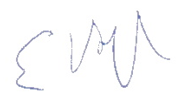
\includegraphics[trim={0 0 0 0},clip,scale=1]{handtek.PNG}
\end{figure}
	    	
	    Begeleider vanuit de Haagse Hogeschool: \emph{J. van Krimpen-Vos}
	\end{flushleft}
	
\end{titlepage}
\sffamily
\newpage
\section*{Voorwoord}
Dit verslag beschrijft de uitvoering van Stage 1 van de opleiding Toegepaste Wiskunde aan de Haagse Hogeschool van de studente Simone Hartgring. \\
De stage is uitgevoerd in opdracht van TNO. Tijdens de stage is een simulatie-omgeving, waarvan de basis door TNO is aangeleverd, zodanig uitgebreid dat hier dreigingsscenario's mee kunnen worden gesimuleerd. Ook is statistisch onderzoek gedaan naar de eigenschappen van mensen die betrokken zijn in dreigingsscenario's en zijn berekeningen uitgevoerd met betrekking tot het gedrag van de betrokkenen. 
\\ \\
Het verslag begint met een beschrijving van het bedrijf, de probleemstelling en de doelstelling in hoofdstuk \ref{intro}. 
In hoofdstuk \ref{opdracht} van het verslag is de opdracht verder toegelicht met een omschrijving en hoofd- en deelvragen.
In hoofdstuk \ref{methode} zijn de methodes die zijn gebruikt bij het uitvoeren van de stageopdracht beschreven. \\
Hoofdstuk \ref{Heigenschappen} bevat een beschrijving van het statistische onderzoek naar eigenschappen van betrokken partijen binnen de dreigingssituaties. Hier zijn ook de resultaten van het onderzoek uitgewerkt en toegelicht. 
In hoofdstuk \ref{gedrag} staat een uitwerking van het onderzoek en de berekeningen met betrekking tot het gedrag van betrokkenen binnen dreigingssituaties. 
De uitbreiding van de simulatie-omgeving is beschreven in hoofdstuk \ref{simulatie}. In dit hoofdstuk staat ook de beginsituatie van de omgeving beschreven. 
De conclusie van het onderzoek staat in hoofdstuk \ref{conclusie}.
Aanbevelingen die de opdrachtgever bij de verdere uitbreiding van de simulatie-omgeving mee kan nemen staan in hoofdstuk \ref{advies}.
Tot slot is in bijlage \ref{reflect} op het verloop van de stage gereflecteerd en is een beschrijving van de behaalde competenties te lezen in bijlage \ref{competenties}.
\\ \\
Graag dank ik Erik Vullings, de opdrachtgever en begeleider vanuit TNO, voor de begeleiding die hij tijdens het verloop van de stage heeft gegeven. \\
Ook gaat mijn dank naar Janine van Krimpen-Vos voor haar begeleiding in zaken met betrekking tot de opleiding.

\newpage
\section*{Samenvatting}
TNO heeft een eenvoudige omgeving ontwikkeld waarin gedrag van bijvoorbeeld mensen gesimuleerd kan worden. Deze wil het bedrijf uiteindelijk gebruiken om de effectiviteit van procedures in dreigingsscenario's te evalueren. De aangeleverde omgeving is nog te eenvoudig om voor het gewenste doel te kunnen worden gebruikt. 
\\
De stagiaire heeft de taak gekregen om de simulatie-omgeving zodanig uit te breiden dat de dreigingsscenario's, die door de opdrachtgever zijn beschreven, gesimuleerd kunnen worden. In de omgeving wordt gebruik gemaakt van agent-based simuleren. Hier krijgen agents, die bijvoorbeeld personen kunnen representeren, eigenschappen en een agenda met taken die de agent tijdens de simulatie uitvoert.
\\ \\
Aan de hand van een statistisch onderzoek is bepaald welke persoonseigenschappen in welke verhoudingen voorkomen bij de groep mensen die verdacht zijn van de volgende misdrijven: Openlijk geweld, aantasting van de openbare orde en het tonen van geweld tegen politieambtenaren. De resultaten van dit onderzoek zijn niet in de simulatie-omgeving verwerkt, maar de opdrachtgever kan de keuze maken om dit tijdens verdere uitbreidingen in de omgeving te verwerken.
\\ \\
Er is een formule bepaald die de snelheid van een groep mensen berekent op basis van de afstand tussen de mensen binnen de groep. Deze formule is in de simulatie-omgeving verwerkt.
\\ \\
Na het toevoegen van nieuwe type agents, eigenschappen, acties en reacties van agents en verbeteringen aan de visualisatie van de simulatie is de omgeving zodanig uitgebreid dat de effecten en acties van betrokkenen in een scenario zichtbaar zijn.
\\Het realisme van het gedrag dat in de simulatie wordt getoond kan verbeterd worden. TNO wordt geadviseerd om onderzoek te doen naar hoe het realisme van het gedrag van worden verbeterd.

\newpage
\tableofcontents
\newpage

\section{Introductie} \label{intro}
\subsection{Het bedrijf} 
De Nederlandse Organisatie voor toegepast-natuurwetenschappelijk onderzoek (TNO) is een zelfstandige onderzoeksorganisatie. Dit houdt in dat het geen onderdeel is van een overheidsinstantie, universiteit of onderneming. De organisatie is opgericht om kennis toepasbaar te maken voor bedrijven en overheden. 
\\ \\
TNO bestaat uit meerdere units die vervolgens uit afdelingen bestaan. Defensie en Veiligheid is één van deze units. De stage is onderdeel van de afdeling Modelling, Simulation \& Gaming binnen Defensie en Veiligheid. Binnen de afdeling worden onder anderen virtuele omgevingen gemodelleerd en realistische simulatiemodellen gemaakt die worden voorzien van menselijk gedrag en interactie met andere systemen. De afdeling heeft een grootte van ongeveer 35 werknemers.
\\ \\
Bij TNO worden verschillende projecten uitgevoerd. Sommige projecten maken onderdeel uit van een overkoepelend programma. Het stageproject is onderdeel van het programma V2018 Adaptief Bewaken \& Beveiligen in stedelijk gebied. Dit programma draagt bij aan het adaptief werken en adequaat samenwerken van de politie en Koninklijke Marechaussee (KMar).
\\ \\
Dit is van belang omdat de omstandigheden waarin de politie en KMar aan bewaken en beveiligen doen vaak veranderen.  Er moeten nieuwe technieken en methoden worden ontwikkeld die ervoor zorgen dat er snel gereageerd kan worden op dreigingen op onverwachte locaties en er meer situationeel inzicht wordt gedaan in verstedelijkte gebieden. De stageopdracht, die later in dit hoofdstuk wordt toegelicht, draagt bij een het geven van inzicht in dreigingsscenario's en biedt de mogelijkheid om hier nieuwe methoden en technieken in te verwerken.

\subsection{Probleemstelling}
TNO heeft een eenvoudige omgeving ontwikkeld waarin gedrag van bijvoorbeeld mensen gesimuleerd kan worden. TNO wil deze omgeving kunnen gebruiken om dreigingsscenario's te simuleren en te bepalen welke procedures en middelen het meest effectief zijn in deze scenario's.\\
Op het moment van de start van de stage was de omgeving hier nog te eenvoudig voor en kon het dus niet voor het gewenste doel worden gebruikt. Daarom moest de omgeving worden uitgebreid met nieuwe gedragingen en reacties van de gesimuleerde mensen. 

\subsection{Doelstelling}
Het doel van de stage is het zodanig uitbreiden van de eerder genoemde simulatie-omgeving dat de door de opdrachtgever aangeleverde scenario's hierin gesimuleerd kunnen worden.




\newpage
\section{Opdracht} \label{opdracht}
\subsection{Opdrachtomschrijving}

TNO beschikt over een eenvoudige simulatie-omgeving. In deze omgeving worden taken toegekend aan zogenoemde agents. Deze agents zijn objecten die mensen, voertuigen of robots representeren. Een voorbeeld is dat iemand naar zijn werk gaat. Bij het runnen van de simulatie is in een webapplicatie te zien hoe de agents zich voortbewegen, dus hoe de persoon uit het voorbeeld naar zijn werklocatie loopt. De visualisatie bestaat uit een kaart waar elk persoon als een icoon op wordt afgebeeld (zie Figuur \ref{voorbeeld visualisatie}).

\begin{figure}[h]
\centering
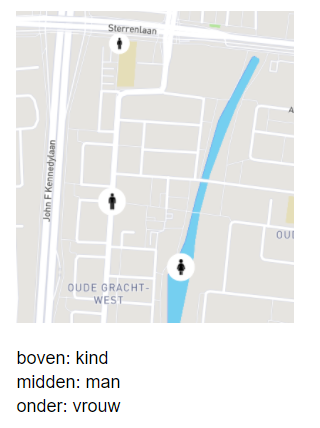
\includegraphics[trim={0 5cm 0 2cm},clip,scale=1]{01.png}
\caption{Voorbeeld van de visualisatie van een simulatie}
\label{voorbeeld visualisatie}
\end{figure}

\noindent Om een complete simulatie van een dreigingsscenario te maken zijn er drie groepen die gesimuleerd moeten worden:
\begin{enumerate}
    \item De agents die de bedreiging vormen (team ROOD).
    \item De agents die de dreiging oplossen, zoals de politie of KMar (team BLAUW).
    \item De rest van de omgeving, zoals omstanders die toevallig aanwezig zijn, maar geen direct onderdeel zijn van de dreiging (team WIT).
\end{enumerate}
De stagiaire heeft de taak gekregen om team ROOD te programmeren. Verder heeft de stagiaire zich bezig gehouden met het loop- en vluchtgedrag en de verschillende soorten agents binnen team WIT. Een voorbeeld van wat onder het programmeren van het loop- en vluchtgedrag valt is het verwerken van de snelheid waarmee de agent zich voortbeweegt. Met de verschillende soorten agents worden naast mensen ook bijvoorbeeld voertuigen en robots bedoeld. 
\\
Een andere stagiaire binnen hetzelfde project heeft de taak om team BLAUW en de communicatie en takenpakketten van team WIT te programmeren. \\ \\
Uiteindelijk wordt de simulatie gebruikt om de effectiviteit van acties van team BLAUW tegen de dreiging die door team ROOD wordt gevormd te testen.

\subsection{Hoofd- en deelvragen}
Het stageproject geeft antwoord op de volgende hoofdvraag: \textbf{Hoe kunnen dreigingsscenario's zodanig worden gesimuleerd dat de effecten en acties van betrokkenen in een scenario zichtbaar zijn?} \\
De opdrachtgever geeft aan welke effecten en acties van betrokkenen zichtbaar moeten zijn in de simulatie.
\\ \\
Om de hoofdvraag te kunnen beantwoorden moet antwoord worden gegeven op de volgende deelvragen:
\begin{enumerate}
    \item Welke dreigingsscenario's moeten gesimuleerd kunnen worden?
    \item Welke eigenschappen moeten volgens statistische toetsen aan personen in de simulatie worden toegekend?
    \item Hoe kan aan de hand van berekeningen het gedrag van de agents geïmplementeerd worden?
    \item Welke acties moeten zichtbaar zijn in de simulatie?
    \item Welke effecten van de toegevoegde acties moeten zichtbaar zijn in de simulatie?
\end{enumerate}
De methode die wordt gebruikt om de deelvragen te beantwoorden is beschreven is hoofdstuk \ref{methode}.
Deelvraag 1 zal in verband met vertrouwelijkheid niet in het verslag worden beantwoord. Het antwoord op deelvraag 2 staat beschreven in hoofdstuk \ref{Heigenschappen}. Deelvraag 3 is beantwoord in hoofdstuk \ref{gedrag}.
De laatste twee deelvragen zijn in hoofdstuk \ref{simulatie} uitgewerkt. 
De hoofdvraag van het onderzoek wordt beantwoord in de conclusie.
\newpage



\section{Methode} \label{methode}
\subsection{Onderzoek naar dreigingsscenario's}
Het eindproduct wordt uiteindelijk gebruikt om dreigingssituaties te simuleren. Om deze zo goed mogelijk te kunnen simuleren is eerst onderzoek gedaan naar onderwerpen die betrekking hebben tot de dreigingssituaties die gesimuleerd worden. 
\\ \\
Dit begon met het verzamelen van data over de eigenschappen van een groep die in een scenario team ROOD zou kunnen vormen. De data is met name afkomstig van de website van het Centraal Bureau van Statistiek (CBS). Na het vinden van genoeg relevante data is met de chi-kwadraat toets bepaald wat de verhoudingen van bepaalde eigenschappen binnen een groep zijn. Vervolgens is met de opdrachtgever bepaald welke van deze eigenschappen worden meegenomen in de simulatie. Het onderzoeken van de juiste verhoudingen zorgt voor een representatieve groep binnen de simulatie, als bijvoorbeeld blijkt dat bij een bepaalde situatie team ROOD voor 80\% uit mensen onder de 25 jaar bestaat zal voor elke agent uit team rood een kans van 0,8 bestaan dat de leeftijd van de agent lager is dan 25. Het uitgevoerde onderzoek staat in hoofdstuk \ref{Heigenschappen} beschreven. \\ \\
Ook is een literatuuronderzoek uitgevoerd naar het gedrag dat aan agents moet worden toegekend. Hier is gezocht naar wetenschappelijke artikelen waarin wordt toegelicht hoe bepaalde gedragingen kunnen worden berekend. Een voorbeeld hiervan is de snelheid waarmee een groep mensen zich voortbeweegt. Met de opdrachtgever is vervolgens afgewogen welke berekeningen mee worden genomen in de simulatie en welke hier te complex voor zijn. Een te complexe formule kan de simulatie namelijk sterk vertragen. De uitgevoerde berekeningen zijn te vinden in hoofdstuk \ref{gedrag}.

\subsection{De simulatie}
\subsubsection{Agent-based simuleren}
De methode waarmee gesimuleerd wordt staat bekend als agent-based simuleren. Dit is een vorm van simuleren waarin de onderdelen (agents) afzonderlijk worden onderzocht. In de simulatie voeren alle agents gelijktijdig hun opgedragen acties uit. Van deze acties kan het effect worden bekeken. Een agent kan bijvoorbeeld een mens zijn die de taak krijgt om een winkel te beroven. De agent voert dit uit en er kan worden gekeken wat het effect hiervan is, bijvoorbeeld dat de politie naar de winkel komt. \\ \\
In dit project representeren de agents voornamelijk mensen die betrokken zijn bij de dreigingssituaties die onderzocht worden door de eindgebruiker. De agents kunnen ook voertuigen of bijvoorbeeld robots representeren. Elke agent krijgt een zogenoemde agenda. Deze agenda is een pakket aan taken dat de agent uit moet voeren, zoals naar werk lopen, werken, boodschappen doen en terug naar huis lopen. Wanneer de simulatie draait worden de taken in de agenda in chronologische volgorde uitgevoerd. \\
Er kunnen situaties ontstaan waarin agents op elkaar reageren. In die situaties worden de agenda’s van de agents tijdens het draaien van de simulatie aangepast naar de situatie. Een voorbeeld hiervan is: Een agent is aan het wandelen. Bij hem in de buurt begint iemand mensen aan te vallen. In plaats van dat de agent blijft wandelen wordt de agenda zodanig aangepast dat de agent de taak krijgt om weg te rennen van de situatie. \\ \\
Het doel van het project is dat dreigingssituaties worden gesimuleerd. Zoals eerder genoemd worden de betrokkenen in drie groepen onderverdeeld: team WIT, team BLAUW en team ROOD.
\begin{itemize}
    \item Team WIT voert het “normale” gedrag uit. De agents uit dit team zullen dus agenda’s krijgen met alledaagse taken zoals naar werk gaan en winkelen.
    \item Team BLAUW voert de taken van de politie en KMar uit. De agenda’s zullen bestaan uit taken als “bewaken” en “patrouilleren”. Het gedrag van team BLAUW zal ook voor een groot deel bestaan als reacties, dus taken die tijdens het draaien van de simulatie aan de agenda worden toegevoegd als reactie op acties van andere agents. Een voorbeeld hiervan is het aanhouden van een agent. Zoals eerder genoemd wordt dit gedrag door een andere stagiaire aan het simulatiemodel toegevoegd.
    \item Team ROOD voert de taken uit die de dreiging vormen. Ook van team ROOD bestaat het gedrag voor een groot deel uit reacties. Een voorbeeld is dat twee agents de taak krijgen om met elkaar te vechten. De andere rode agents die in de buurt staan kunnen dan als reactie deelnemen aan het gevecht of weglopen.
\end{itemize}
Naast agenda's krijgen de agents ook eigenschappen, zoals een geslacht. Deze eigenschappen kunnen ook bepalen hoe een agent op bepaalde acties reageert. Een eigenschap van een agent kan bijvoorbeeld zijn tot welke van de eerder genoemde teams hij behoort. Als de agent bij team BLAUW hoort zal hij anders reageren op dreigingen dan als hij bij team WIT zou horen. 

\subsubsection{Uitbreiden van de simulatie-omgeving}
Het uitbreiden van de simulatie-omgeving is in een aantal stappen uitgevoerd:
\begin{enumerate}
    \item Om te kunnen beginnen met het uitbreiden van de simulatie-omgeving moet de omgeving kunnen draaien op de laptop van de stagiaire. Hiervoor heeft de stagiaire de juiste programma's en bestanden geïnstalleerd en gedownload. De geïnstalleerde programma's zijn GitHub Desktop\footnote{GitHub wordt gebruikt om de geschreven code met anderen te kunnen delen},Visual Studio Code\footnote{VS Code is de editor die tijdens het project wordt gebruikt}, Docker \footnote{Docker is een programma dat wordt gebruikt om softwarepakketten op de achtergrond uit te voeren} en node.js \footnote{node.js is de gebruikte run-time omgeving}.
    \item Het uitbreiden start met het toevoegen van nieuwe type agents en taken en agenda's. Een voorbeeld van een nieuw type agent is een agent die een groep representeert.
    \item Hierna is stap 2 aangepast en uitgebreid naar de dreigingsscenario's. In deze stap zijn dus taken en agents toegevoegd die betrekking hebben tot bepaalde dreigingsscenario's.
    \item Voor elk dreigingsscenario is een configuratiebestand gemaakt. Dit is een bestand waarin staat welke agents met welke eigenschappen voor het scenario gegenereerd moeten worden. Wanneer een agent een specifieke agenda moet krijgen is dit ook in het configuratiebestand gezet. Er is een stuk code aan de simulator toegevoegd die de op basis van de gegevens uit het configuratiebestand de juiste agents en agenda's genereert. Het werken met configuratiebestanden zorgt voor duidelijk onderscheid tussen de scenario's en op deze manier kan gemakkelijk tussen de verschillende scenario's gewisseld worden.
\end{enumerate}

\newpage
\section{Onderzoek naar eigenschappen} \label{Heigenschappen}
In dit hoofdstuk staat het onderzoek naar eigenschappen van betrokkenen in dreigingssituaties beschreven. Het gaat hier om algemene dreigingen die vaak met het eindproduct bekeken zullen worden. Hieronder vallen openlijk geweld en aantasting van de openbare orde. In de simulaties wordt er ook rekening mee gehouden dat er mensen zullen zijn die zich verzetten tegen de politie en KMar. \\ \\
De eigenschappen geslacht, leeftijd, samenstelling van het huishouden, inkomens-percentiel en de stedelijkheidsklasse kunnen in berekende verhoudingen (te zien in tabel \ref{res02} in bijlage \ref{tabellen}) in de simulatie worden meegenomen. Hoe deze eigenschappen geselecteerd zijn en wat de verhoudingen zullen zijn per dreiging is in het hoofdstuk uitgewerkt.

\subsection{Literatuuronderzoek}
Om het onderzoek uit te kunnen voeren is eerst data verzameld. Deze data is met name gezocht op de site van het Centraal Bureau van Statistiek. Een referentie naar de gevonden datasets is te vinden in bijlage \ref{bronnencbs}.

\subsubsection{Openlijk geweld \& aantasting openbare orde} \label{dataset1}
Elk jaar publiceert het CBS data over verdachten van misdrijven. In deze bestanden staat onder anderen data over de verdachten van openlijk geweld en van aantasting van de openlijke orde. \\
Voor dit onderzoek is de data van de jaren 2018, 2019 en 2020 met elkaar vergeleken om een algemene conclusie te trekken. \\ \\
In het databestand (Centraal Bureau voor de Statistiek, 2021) staat per persoonseigenschap en per misdrijf het aantal mensen dat in Nederland in het bekeken jaartal verdacht is geweest van het misdrijf. De misdrijven waar in dit hoofdstuk de focus op ligt zijn het tonen van openlijk geweld en het aantasten van de openbare orde. \\ \\
De persoonseigenschappen die in deze dataset staan en waar de statistische toetsen op zijn uitgevoerd zijn te verdelen in de categorieën ``geslacht, ``leeftijd'', ``samenstelling van het huishouden'', ``inkomens-percentiel'', ``stedelijkheidsklasse'', ``hoogst behaalde opleiding'' en de ``migratieachtergrond''. \\
Om een beeld te geven van hoe deze dataset eruit ziet is in Tabel \ref{CBS01} het deel van de dataset te zien waar de verhoudingen van de eigenschappen ``man'' en ``vrouw'' in het jaar 2018 voor de genoemde misdrijven zichtbaar is:

\begin{table}[h]
\begin{center}
\caption{Onderdeel dataset Openlijk geweld \& Aantasting openbare orde}
 \begin{tabular}{|r|c c|} 
 \hline
  & man & vrouw \\ 
 \hline\hline
 Openlijk geweld & 4730 & 720 \\ 
 \hline
 Aantasting van de openbare orde & 5110 & 450 \\
 \hline
\end{tabular}
\label{CBS01}
\end{center}
\end{table}
 
\noindent In 2018 zijn dus 4730 mannen en 720 vrouwen geregistreerd als verdachten van openlijk geweld.

\subsubsection{Geweld tegen politieambtenaren}
In 2019 heeft het Centraal Bureau van Statistiek een onderzoek gedaan naar de eigenschappen van verdachten van geweld en agressie tegen politieambtenaren. Wegens een tekort aan data van andere jaren wordt ervan uit gegaan dat de data uit 2019 nog steeds representatief is. \\ \\
In het databestand (Centraal Bureau voor de Statistiek, 2020) staat per persoonseigenschap het aantal mensen dat in 2019 verdacht is geweest van geweld en agressie tegen politieambtenaren. Het gaat om dezelfde persoonseigenschappen als in de dataset die in paragraaf \ref{dataset1} wordt genoemd. Een onderdeel van de dataset, waar de verhouding van de eigenschappen ``man'' en ``vrouw'' binnen de groep van verdachten van het tonen van geweld tegen politieambtenaren wordt beschreven, is in Tabel \ref{CBS02} te zien. 

\begin{table}[h]
\begin{center}
\caption{Onderdeel dataset Geweld tegen politieambtenaren}
 \begin{tabular}{|r|c|} 
 \hline
  & verdachten\\ 
 \hline\hline
 mannen & 4510 \\ 
 \hline
 vrouwen & 570 \\
 \hline
\end{tabular}
\label{CBS02}
\end{center}
\end{table}
 
\noindent In 2019 zijn dus 4510 mannen en 570 vrouwen geregistreerd als verdachten van geweld tegen politieambtenaren.

\subsection{Data Analyse}
De data, verkregen uit het literatuuronderzoek, is geanalyseerd om tot een conclusie te kunnen komen over de eigenschappen van de verdachten. Dit begon met het groeperen van de data. Vervolgens is per groepering de homogeniteit van de data getoetst met behulp van de chi-kwadraattoets.
\subsubsection{Data Groeperen}
De data is per categorie van eigenschappen gegroepeerd. Met een categorie wordt bijvoorbeeld bedoeld dat de eigenschappen “man” en “vrouw” behoren tot de categorie “geslacht”. Dit is gedaan met behulp van het programma RStudio. Voor elke categorie is een subset gevormd.
\subsubsection{Homogeniteit toetsen}
De chi-kwadraattoets voor homogeniteit gaat uit van homogeniteit. Dit houdt in dat elke eigenschap binnen een categorie een gelijke heeft. Bij bijvoorbeeld de subset voor de categorie “geslacht”: De chi-kwadraattoets gaat ervan uit dat er evenveel mannen als vrouwen verdacht zijn. Dat zou betekenen dat het geslacht geen invloed heeft op het deelnemen aan het onderzochte misdrijf.\\
De chi-kwadraattoets berekent het totaal van de gewogen kwadratische afwijkingen tussen de aantallen in de dataset en de aantallen als er sprake zou zijn van homogeniteit. Als dit totale aantal te groot is wordt de hypothese dat er sprake is van homogeniteit verworpen. 
\\ \\
De chi-kwadraattoets wordt met de volgende code in RStudio uitgevoerd:
\begin{center}
    \begin{tabular}{|c|} 
        \hline
        {\fontfamily{qcr}\selectfont
        >chisq.test(subset)
        } \\
        \hline
    \end{tabular}
\end{center}
Het uitvoeren van deze code resulteert in een p-waarde. Een p-waarde van 0,05 of hoger geeft aan dat er sprake is van homogeniteit. Een p-waarde lager dan 0,05 geeft aan dat het totaal van de gewogen kwadratische afwijkingen te hoog is en er geen sprake is van homogeniteit. De eigenschap heeft dan dus invloed op de waarschijnlijkheid dat een persoon als verdacht wordt gezien.
\\
Wanneer er geen sprake is van homogeniteit worden de verhoudingen van de eigenschappen in de dataset berekend om tot een conclusie te komen over de eigenschappen van de verdachten.
\subsection{Resultaten}
\noindent In de resultaten is de laagste waarde hoger dan 0 die RStudio bij het uitvoeren van de chi-kwadraattoets toont gelijk aan $2,2\mathrm{e}{-16}$. Wanneer deze waarde wordt gegeven betekent dit dus dat de waarde ook lager kan zijn dan $2,2\mathrm{e}{-16}$.
\\
De p-waarden die zijn verkregen door het uitvoeren van de chi-kwadraattoets voor homogeniteit in RStudio zijn , zoals verwerkt is in Tabel \ref{res01} in Bijlage \ref{tabellen}, elk gelijk aan $2,2\mathrm{e}{-16}$. Er is dus bij elke eigenschap sprake van homogeniteit. De verhoudingen van de eigenschappen zijn dus voor elke categorie berekend.
\\
Dit is gedaan door per eigenschap binnen een categorie het aantal verdachten te delen door het totaal aantal verdachten binnen de categorie. Vervolgens is dit getal vermenigvuldigd met 100. Wanneer er meerdere jaren onderzocht worden is de gemiddelde waarde van alle jaren berekend.\\
De resultaten hiervan zijn in Tabel \ref{res02} in Bijlage \ref{tabellen} te zien.
\\ \\
In deze resultaten valt op dat met name het geslacht een grote invloed lijkt te hebben op de betrokkenheid van iemand in een misdrijf. Mannen vormen bij elk onderzochte misdrijf de grote meerderheid.

\subsection{Conclusies over de resultaten}
Na overleg met de opdrachtgever is besloten om de categorieën “Migratie achtergrond” en “Hoogst behaalde opleiding” niet in de simulatie mee te nemen. De reden hiervoor is dat er binnen de dataset sprake kan zijn van vooroordelen of dat de resultaten de vooroordelen kunnen versterken. 
\\ \\
Voor de categorie"en "geslacht", "leeftijdsklasse", “Samenstelling huishouden”, “Inkomenspercentiel” en “Stedelijkheidsklasse” kunnen de berekende verhoudingen van de eigenschappen in de simulatie verwerkt worden.
\\ Tijdens de stage was er niet genoeg tijd om de verhoudingen in de simulatie te verwerken. Wel wordt de opdrachtgever geadviseerd om de verhoudingen in verder onderzoek mee te nemen.

\newpage
\section{Onderzoek naar gedrag} \label{gedrag}
Met de opdrachtgever is besproken welk gedrag door de stagiaire onderzocht moet worden. De focus van het onderzoek ligt op de snelheid waarmee een groep zich voortbeweegt. Na het uitvoeren van literatuuronderzoek is bekeken hoe het onderzoek het best in de simulatie kan worden toegepast zonder de simulatie significant te vertragen.
\\ \\
In veel dreigingssituaties spelen grote groepen mensen een rol. Een voorbeeld hiervan is een demonstratie. De hypothese is dat een grotere groep mensen zich met een lagere snelheid voortbeweegt dan een kleinere groep. In dit hoofdstuk staat beschreven hoe tot een formule voor de snelheid van een groep is gekomen.
\subsection{Literatuuronderzoek}

Volgens meerdere onderzoeken naar het simuleren van groepen (Helbing et al., 2000), (Leijonmarck \& Olergård, 2013) \& (Thio, 2019)) kan de versnelling waarmee een persoon in een groep voortbeweegt worden vertaald in de volgende formule:
\begin{equation} \label{hoofdeq}
    m_{i} \frac{dv_{i}}{dt} = m_{i} \frac{v_{i}^{0}(t)e_{i}^{0}(t) - v_{i}(t)e_{i}(t)}{\tau_{i}} + \displaystyle\sum_{j \neq i} f_{ij} + \displaystyle\sum_{W} f_{iW}
\end{equation}
\begin{center}
\begin{itemize}
\centering
    \item $m_{i} \frac{dv_{i}}{dt}$ : Hierbij is $m_{i}$ de massa van agent $i$ en $\frac{dv_{i}}{dt}$ de versnelling.
    \item $ m_{i} \frac{v_{i}^{0}(t)e_{i}^{0}(t) - v_{i}(t)}{\tau_{i}}$ geeft de gewenste versnelling weer. Hier is $v_{i}^{0}(t)$ de \\ gewenste snelheid op moment $t$, $e_{i}^{0}(t)$ de gewenste bewegingsrichting en $v_{i}(t)$ \\ en $e_{i}(t)$ de daadwerkelijke snelheid en richting. $\tau_{i}$ is de tijdstap waarmee gerekend wordt.
    \item $\displaystyle\sum_{j \neq i} f_{ij}$ geeft de interactie weer tussen agent $i$ en agent $j$.
    \item $\displaystyle\sum_{W} f_{iW}$ geeft de interactie weer tussen agent $i$ en muur $W$.
\end{itemize}
\end{center}

De formules voor de interactie tussen twee agents en tussen een agent en een muur zien er als volgt uit:
\begin{equation}\label{eqagents}
\mathbf{f}_{i j}=\left\{ {\color{blue} A_{i} \exp \left[\left(r_{i j}-d_{i j}\right) / B_{i}\right]}+{\color{ForestGreen}k g\left(r_{i j}-d_{i j}\right)}\right\} \mathbf{n}_{i j}+{\color{red}\kappa g\left(r_{i j}-d_{i j}\right) \Delta v_{j i}^{t} \mathbf{t}_{i j}}
\end{equation}
\begin{equation}\label{eqmuur}
\begin{aligned}
\mathbf{f}_{i W}=&\left\{ {\color{blue}A_{i} \exp \left[\left(r_{i}-d_{i W}\right) / B_{i}\right]}+{\color{ForestGreen}k g\left(r_{i}-d_{i W}\right)}\right\} \mathbf{n}_{i W}-{\color{red}\kappa g\left(r_{i}-d_{i W}\right)\left(\mathbf{v}_{i} \cdot \mathbf{t}_{i W}\right) \mathbf{t}_{i W}}
\end{aligned}
\end{equation}

\noindent Het {\color{blue}blauwe deel} van de formules representeert de drang van mensen om van elkaar of van een muur weg te blijven. Hierbij zijn A en B constanten, is $r_i$ de straal van agent $i$, $r_{ij}$ de som van de straal van agent $i$ en van agent $j$ en $d$ de afstand tussen agent $i$ en agent $j$ of tussen agent $i$ en muur $W$.\\ \\
Het {\color{ForestGreen} groene deel} in de formules geeft de kracht weer die twee mensen van elkaar weg duwt bij een aanraking. Wanneer er geen aanraking plaatsvindt krijgt $g$ de waarde $0$, als er wel sprake is van aanraking is deze gelijk aan $1$. In de formules is k een constante. \\
De waarde $n$ is de genormaliseerde vector van agent $j$ naar agent $i$ of van muur $W$ naar agent $i$. \\ \\
Het {\color{red}rode deel} in de formule geeft de wrijving weer die ontstaat wanneer een agent een andere agent of een muur aanraakt. Wederom is $g$ gelijk aan $1$ bij aanraking en gelijk aan $0$ bij afwezigheid van aanraking. De waarde $\kappa$ is een constante.\\ Het laatste deel van de formule ($\Delta v_{j i}^{t} t_{i j}$ of $(v_{i} \cdot t_{i W}) t_{i W}$) is de vector in tangentiële richting. \\Het verschil tussen de groene en rode kracht is in Figuur \ref{krachten1} weergegeven, waar de kleuren van de vectoren (groen en rood) gelijk staan aan de kleuren van de krachten binnen de formule. 
\\
\begin{figure}[h]
\centering
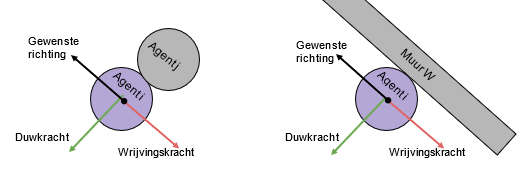
\includegraphics[scale=1]{02.png}
\caption{Verschillende krachten bij contact van een agent}
\label{krachten1}
\end{figure}

\noindent Een aantal waarden in de formule, zoals die van de constanten, staan al vast. Dit zijn de volgende waarden:
\begin{center}
    $A_i$ : $2 \cdot 10^3$ N \\
    $B_i$ : $0,08$ m \\
    $\tau_i$ : $1$ s \\
    $k$ : $1,2 \cdot 10^5 \text{ kg s}^{-2}$ \\
    $\kappa$ : $2,4 \cdot 10^5 \text{ kg m}^{-1}\text{s}^{-1}$ \\
    $m_i$ : $80$ kg\\
    $v_i^{0}(t)$ : $1,4$ m/s \\
    $r_i$ : $0,175$ m
\end{center}
\subsection{Berekeningen}
In de simulatie wordt een groep gerepresenteerd door een agent. De mensen in een groep worden dus niet apart gesimuleerd en het is dan ook niet mogelijk om per agent de versnelling te berekenen. Daarom wordt tijdens de volgende berekeningen gezocht naar de versnelling van de volledige groep, gebaseerd op de dichtheid van een groep.
\\ \\
De berekeningen worden uitgevoerd voor een agent die zich binnen de groep bevindt, dus niet aan de randen van de groep. Om deze reden wordt in de berekeningen geen rekening gehouden met muren en wordt formule \ref{eqmuur} niet gebruikt. Er wordt vanuit gegaan dat de versnelling binnen de groep representatief is voor de gehele groep.\\
Er wordt uitgegaan van dichtheden waarbij agents elkaar niet aanraken. Van formule \ref{eqagents} blijft dan alleen het blauwe deel over. In dit deel van de formule, het deel dat de drang om van andere mensen weg te blijven representeert, houdt alleen rekening met mensen in het gezichtsveld van de agent. Als een agent iemand niet kan zien ontstaat er immers ook geen drang om van deze agent weg te blijven.

\subsubsection{Versnelling}
Het eerste deel na het =-teken van formule \ref{hoofdeq}, waar de gewenste snelheid en gewenste bewegingsrichting worden meegenomen, geeft bij invullen van de eerder genoemde vaste waarden het volgende:
\begin{equation}\label{01eq}
    m_{i} \large \frac{v_{i}^{0}(t)e_{i}^{0}(t) - v_{i}(t)e_{i}}{\tau_{i}} =  \normalsize 80 \large \frac{1,4 [ \begin{smallmatrix}  0 \\ 1 \end{smallmatrix} ]- v_{i}(t) \cdot\left[\begin{array}{l}
0 \\
1
\end{array}\right]}{1}
\end{equation} 
Om de berekeningen te versimpelen worden alleen de agents direct naast, voor en schuin voor de agent gezien als agents die binnen het gezichtsveld vallen. Dit zijn in totaal 5 agents. In Figuur \ref{gezichtsveld} is dit weergegeven.
\\ 
\begin{figure}[h]
\centering
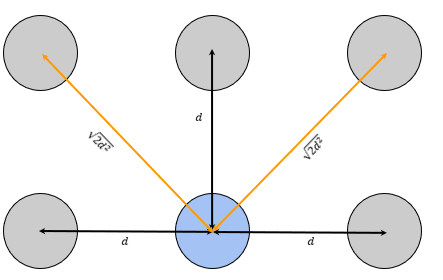
\includegraphics[scale=1]{03.png}
\caption{Agents die worden gezien als binnen het gezichtsveld van agent i}
\label{gezichtsveld}
\end{figure}

\noindent Dit geeft bij het invullen van de vaste waarden in formule \ref{eqagents} de volgende berekening:
\begin{equation}\label{02eq}
    \begin{aligned}
        &\sum\left(A_{i} \exp \left[\frac{\left(r_{i j}-d_{i            j}\right)}{B_{i}}\right] \cdot n_{i j}\right) \\
        &=\left(2 \cdot 10^{3} \cdot \exp     \left[\frac{(0,36-d)}{0,08}\right]\right)     \cdot\left[\begin{array}{c}
            1 \\
            0
        \end{array}\right]+\left(2 \cdot 10^{3} \cdot \exp     \left[\frac{(0,36-d)}{0,08}\right]\right)    \cdot\left[\begin{array}{c}
            0 \\
            -1
        \end{array}\right] \\
        &+\left(2 \cdot 10^{3} \cdot \exp     \left[\frac{(0,36-d)}{0,08}\right]\right)     \cdot\left[\begin{array}{c}
            -1 \\
            0
        \end{array}\right]+\left(2 \cdot 10^{3} \cdot \exp     \left[\frac{\left(0,36-\sqrt{2     d^{2}}\right)}{0,08}\right]\right)             \cdot\left[\begin{array}{c}
            \frac{\sqrt{2}}{2} \\
            -\frac{\sqrt{2}}{2}
        \end{array}\right] \\
        &+\left(2 \cdot 10^{3} \cdot \exp         \left[\frac{\left(0,36-\sqrt{2         d^{2}}\right)}{0,08}\right]\right)         \cdot\left[\begin{array}{c}
            -\frac{\sqrt{2}}{2} \\
            -\frac{\sqrt{2}}{2}
        \end{array}\right] \\
        &=\left(2 \cdot 10^{3} \cdot \exp     \left[\frac{(0,36-d)}{0,08}\right]\right)       \cdot\left[\begin{array}{c}
            0 \\
            -1
        \end{array}\right]+\left(2 \cdot 10^{3} \cdot \exp \left[\frac{\left(0,36-\sqrt{2     d^{2}}\right)}{0,08}\right]\right)            \cdot\left[\begin{array}{c}
            0 \\
            -\sqrt{2}
        \end{array}\right]
    \end{aligned}
\end{equation}
Het samenvoegen van berekeningen \ref{01eq} en \ref{02eq} geeft: 
\begin{equation}
    \begin{aligned}
        &a= \frac{d v_{i}}{d t} = \frac{1,4 [ \begin{smallmatrix}  0 \\ 1 \end{smallmatrix} ]- v_{i}(t)}{1} + \\& \frac{1}{80} \cdot\left(\left(2 \cdot 10^{3} \cdot \exp     \left[\frac{(0,36-d)}{0,08}\right]\right)     \cdot\left[\begin{array}{c}
            0 \\
            -1
        \end{array}\right]+\left(2 \cdot 10^{3} \cdot \exp  \left[\frac{\left(0,36-\sqrt{2             d^{2}}\right)}{0,08}\right]\right)             \cdot\left[\begin{array}{c}
            0 \\
            -\sqrt{2}
        \end{array}\right]\right)
    \end{aligned}
\end{equation}
\\
Om dit perspectief te geven: wanneer de afstand tussen agents in een groep 1,35 meter is (dus schouder tot schouder 1 meter) is de vertraging van de groep in de beginsituatie, waar de snelheid nog gelijk is aan de gewenste snelheid, ongeveer gelijk aan $-9,33 \cdot 10^{-5}$ m/s². In figuur \ref{versnelling} is voor meer onderlinge afstanden de bijhorende vertraging in de beginsituatie te zien. Met vertraging wordt bedoeld dat dit een versnelling is met een negatieve waarde, dus een vertraging van 1 geeft een versnelling van -1 aan.
\begin{figure}[H]
\centering
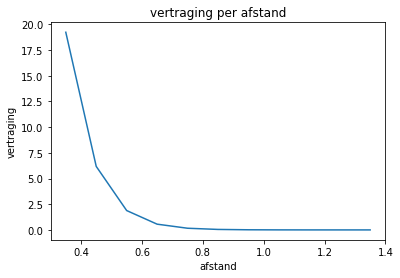
\includegraphics[scale=1]{vertraging.png}
\caption{vertraging}
\label{versnelling}
\end{figure}

\noindent In figuur \ref{versnelling} is te zien dat een kortere onderlinge afstand een grotere vertraging geeft. 
\subsubsection{Snelheid}
Door de negatieve versnelling wordt de daadwerkelijke snelheid lager dan de gewenste snelheid. Daardoor komt in het eerste deel van de formule een positieve waarde uit die invloed heeft op de versnelling. Uiteindelijk zorgt dit voor een versnelling van 0. In dit geval is de uiteindelijke snelheid van de groep bereikt.
\\ \\
De uiteindelijke snelheid wordt bereikt wanneer formule \ref{01eq} gelijk is aan formule \ref{02eq} vermenigvuldigd met -1. Wat deze snelheid moet zijn kan als volgt worden berekend:
\begin{equation}
\begin{gathered}
m_{i} \frac{v_{i}^{0}(t) e_{i}^{0}(t)-v_{i}(t)}{\tau_{i}}=-\sum\left(A_{i} \exp \left[\frac{\left(r_{i j}-d_{i j}\right)}{B_{i}}\right] \cdot n_{i j}\right) \\ 
80 \cdot \frac{1,4 \cdot\left[\begin{array}{l}
0 \\
1
\end{array}\right]-v \cdot\left[\begin{array}{l}
0 \\
1
\end{array}\right]}{1}=\left(2 \cdot 10^{3} \cdot \exp \left[\frac{(0,36-d)}{0,08}\right]\right) \cdot\left[\begin{array}{l}
0 \\
1
\end{array}\right]+ \\ \left(2 \cdot 10^{3} \cdot \exp \left[\frac{\left(0,36-\sqrt{2 d^{2}}\right)}{0,08}\right]\right) \cdot \sqrt{2} \cdot\left[\begin{array}{l}
0 \\
1
\end{array}\right]
\end{gathered}
\end{equation}
\begin{equation}
\begin{gathered}
v=1,4-\frac{1}{80} \cdot \left(\left(2 \cdot 10^{3} \cdot \exp \left[\frac{(0,36-d)}{0,08}\right]\right)-\sqrt{2} \cdot\left(2 \cdot 10^{3} \cdot \exp \left[\frac{\left(0,36-\sqrt{2 d^{2}}\right)}{0,08}\right]\right)\right)
\end{gathered}
\end{equation}

\noindent In figuur \ref{snelheid} is voor verschillende onderlinge afstanden de bijhorende snelheid te zien. De afstand die in dit figuur wordt aangegeven is van middelpunt tot middelpunt (dus niet van schouder tot schouder). Een kleinere onderlinge afstand resulteert in een lagere snelheid.

\begin{figure}[H]
\centering
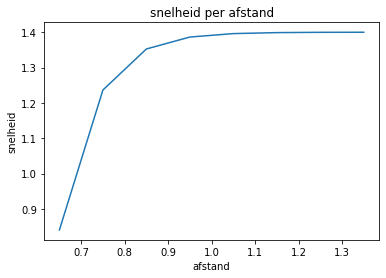
\includegraphics[scale=1]{snelheid3.png}
\caption{snelheid}
\label{snelheid}
\end{figure}

\subsection{Implementatie in het model}
In het simulatiemodel worden grote groepen gerepresenteerd door één agent. De reden hiervoor is dat het werken met losse agents in plaats van een agent voor de gehele groep zou de simulatie significant vertragen en zou ervoor zorgen dat het limiet van het aantal agents dat het model kan verwerken sneller wordt bereikt. \\
Het type agent dat een groep representeert, waar in paragraaf \ref{alg uitbr} meer over wordt toegelicht, krijgt als eigenschap het aantal personen binnen de groep mee. Het oppervlak dat de groep inneemt wordt echter niet meegegeven, waardoor de afstand tussen de personen in de groep niet kan worden bepaald.  Om deze reden wordt een aantal regels opgesteld die de afstand tussen mensen in een groep bepalen:
\begin{itemize}
    \item In groepen kleiner dan 10 mensen is de afstand tussen de mensen binnen de groep van schouder tot schouder gelijk aan 1 meter.
    \item In groepen van 100 tot 250 mensen is de onderlinge afstand gelijk aan 0,8 meter.
    \item In groepen van 250 tot 500 mensen is de onderlinge afstand gelijk aan 0,65 meter.
    \item In groepen van 500 tot 1000 mensen is de onderlinge afstand gelijk aan 0,5 meter.
    \item In groepen van 1000 mensen en groter is de onderlinge afstand gelijk aan 0,3 meter.
\end{itemize}
Er wordt uitgegaan van een invloed van de aanwezigheid van paniek op de afstand tussen mensen in een groep. Bij meer paniek is de afstand tussen mensen kleiner. De agents krijgen een paniek-factor met een waarde tussen 1 en 100. De waarde van deze factor is afhankelijk van de dreiging die in het scenario aanwezig is. Dit wordt verder toegelicht in paragraaf \ref{dreig uitbr}. Voor de invloed van de paniek factor zijn de volgende regels vastgesteld: 
\begin{itemize}
    \item Bij een paniek-factor met een waarde hoger dan 50 en kleiner dan of gelijk aan 70 neemt de onderlinge afstand met 0,1 meter af.
    \item Bij een paniek-factor met een waarde hoger dan 70 en kleiner dan of gelijk aan 90 neemt de onderlinge afstand met 0,2 meter af.
    \item Bij een paniek-factor met een waarde hoger dan 90 neemt de onderlinge afstand met 0,3 meter af.
\end{itemize}
De regels van de onderlinge afstand tussen mensen binnen een groep zijn gebaseerd op eigen ervaring binnen grote groepen en een inschatting op basis van hoeveel mensen naast elkaar lopen en hoe breed een gemiddelde straat is.
\\ \\
De gewenste snelheid van een groep is in het algemeen gelijk aan 5 km/h. Dit is de standaard loopsnelheid van een volwassen mens. De snelheid van de langzaamste persoon in de groep wordt echter aangehouden. Om deze reden wordt wanneer een kind in de groep aanwezig is in de simulatie een lagere snelheid als gewenste snelheid aangehouden, namelijk 3 km/h.  Wanneer een groep aan het rennen is, bijvoorbeeld om te vluchten, wordt deze gewenste snelheid verdubbeld.
\\ \\
Het kan voorkomen dat de berekende snelheid gelijk is aan 0 of zelfs een negatieve waarde krijgt. Het is niet realistisch dat mensen stil blijven staan of achteruit lopen wanneer de groep voortbeweegt. Daarom krijgt de snelheid een minimale waarde van 1 km/h. 

\newpage
\section{De simulatie-omgeving}\label{simulatie}
In dit hoofdstuk wordt de uiteindelijke simulatie-omgeving beschreven. Dit begint met het beschrijven van de beginsituatie, dus wat in de simulatie-omgeving aanwezig was op het moment dat de stage begon. Hierna wordt verteld wat de stagiaire als voorbereidend werk heeft moeten uitvoeren om met de omgeving te kunnen werken. Tot slot wordt beschreven wat de stagiaire aan de omgeving heeft toegevoegd. Toevoegingen die wel in de stageperiode hebben plaatsgevonden, maar door de andere stagiaire zijn toegevoegd (dus team BLAUW en communicatie en geautomatiseerde agenda's van team WIT) worden niet beschreven.
\subsection{De beginsituatie}
De basis van de simulatie-omgeving, die aan het begin van de stage door TNO is aangeleverd, zag er als volgt uit:
\begin{itemize}
    \item In de basis zijn al agents geprogrammeerd en taken die de agents kunnen uitvoeren. Deze taken zijn “naar werk gaan”, “winkelen”, “lunchen”, “werken” en “naar huis gaan”. 
    \item Er is een functie geprogrammeerd die een opgegeven aantal agents genereert met elk een willekeurig gekozen werklocatie. De agents die gegenereerd worden zijn in de beginstand allemaal mannen.
    \item Een agent kan als eigenschap een specifieke auto en/of fiets bezitten. Als het voertuig dicht bij de agent staat gebruikt de agent automatisch het voertuig om bij zijn bestemming te komen.
    \item Bij het runnen van de simulatie worden de agents afgebeeld op een kaart in een webapplicatie. Hier zijn de agents te zien als grijze stippen met een icoon in het midden. Tot nu toe hebben mannen en auto’s een icoon. Voertuigen bewegen met een hogere snelheid op de kaart dan mensen. Als in de webapplicatie op een man wordt geklikt verschijnen een aantal eigenschappen van de agent in het scherm.
    \item Er bestaan functies die een gegeven aantal uren of minuten omzetten naar de tijdseenheid die in de simulatie wordt gebruikt, namelijk milliseconden.
    \item Aan een taak kan een begintijd mee worden gegeven. De agent wacht dan tot de begintijd bereikt is met het uitvoeren van de taak.
    \item Er bestaat een functie die een willekeurige locatie selecteert binnen een gegeven afstand van een gegeven agent. Aan de locatie kan een type worden meegegeven, zodat bijvoorbeeld specifiek een winkel geselecteerd wordt.
    
    \item Het model maakt gebruik van een service (OSRM) die loop-, fiets- en autoroutes kent. Hierdoor nemen de agents een realistische route en bewegen ze bijvoorbeeld niet door gebouwen heen. Dit zorgt er ook voor dat voertuigen op locaties staan waar ze ook daadwerkelijk kunnen staan, een auto staat bijvoorbeeld op de straat van het huis van de agent geparkeerd in plaats van in het huis. 
\end{itemize}
\subsection{Voorbereidend werk}
Om de simulatie-omgeving te kunnen draaien heeft de stagiaire Docker, GitHub Desktop en Visual Studio Code op haar laptop geïnstalleerd. Ook zijn de juiste pakketten van de OSRM service gedownload.\\ \\
De simulaties zijn geprogrammeerd in de taal TypeScript. Dit is een variant van JavaScript waarbij specifieke types aan variabelen worden gebonden. Om bekend te raken met de taal heeft de stagiaire een online cursus gevolgd op de site Codecademy. Deze cursus bestaat uit zes lessen en duurt in totaal ongeveer 10 uur. \\ \\
Voor het visualiseren van de simulaties wordt gebruik gemaakt van CSS. Ook hiervoor heeft de stagiaire een cursus gevolgd op Codecademy. Om aan deze cursus te kunnen starten heeft de stagiaire eerst een cursus HTML gevolgd, ook op Codecademy. De cursus HTML bestaat uit vier lessen en duurt ongeveer 9 uur en de CSS cursus bestaat uit  zes lessen en duurt in totaal ongeveer 10 uur.
\subsection{Uitbreidingen}
Het uitbreiden van de simulatie-omgeving begon met het compleet maken van het "normale gedrag". Hieronder vallen acties van team WIT die geen reactie zijn op dreigingen, het uitbreiden van het vervoer en het toevoegen van nieuwe agent types. \\
Hierna zijn type agents, eigenschappen, acties en reacties toegevoegd die te maken hebben met dreigingsscenario's. Dit zijn met name acties en type agents van team ROOD en vluchtgedrag van team WIT.
\\ \\
In dit hoofdstuk zijn voorbeelden gegeven in de vorm van schermafbeeldingen van de visualisatie van de simulaties. In een aantal van deze afbeeldingen is een grijs vlak met een stip toegevoegd om locaties aan te geven. Deze grijze onderdelen zijn in de werkelijke visualisatie niet te zien.
\subsubsection{Algemene uitbreidingen} \label{alg uitbr}
\textbf{Visualisatie}
\begin{itemize}
    \setlength\itemsep{1.5em}
    \item De agents hebben een eigenschap genaamd \textbf{"force"} gekregen. Deze eigenschap geeft aan tot welk team de agent behoort (dus WIT, ROOD of BLAUW)
        \begin{list}{$\circ$}{}  
            \item In de visualisatie krijgt de cirkel die de agent weergeeft de kleur van het team dat aan de agent is toegekend. Dit is in figuur \ref{01} te zien.
        \end{list}
    \begin{figure}[H]
        \centering
            \fbox{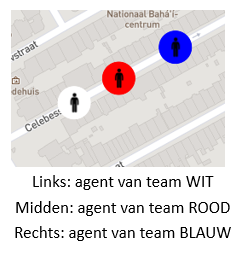
\includegraphics[trim={0 0.5cm 0 0}, clip, scale=1]{sim1.png}}
        \caption{Visualisatie verschillende teams}
        \label{01}
    \end{figure}
    
    \item De \textbf{agent types} "man", "woman", ``girl'' en "boy" \ bestonden al in de basis van de simulatie-omgeving, maar enkel "man" \ werd op dat moment gevisualiseerd. Dit is zodanig uitgebreid dat al deze types gevisualiseerd worden zoals in figuur \ref{02} te zien is: 
        \begin{list}{$\circ$}{}  
            \item Er is een icoon voor een vrouw toegevoegd. Een agent van type "woman" \ wordt gevisualiseerd als een cirkel met in het midden dit icoon.
            \item Een agent van het type "boy" \ krijgt hetzelfde icoon als het type "man", maar in een kleiner formaat. Ook is de cirkel die de agent visualiseert kleiner.
            \item Een agent van het type "girl" \ krijgt hetzelfde icoon als het type "woman", maar in een kleiner formaat. Ook is de cirkel die de agent visualiseert kleiner.
        \end{list}
     \begin{figure}[H]
        \centering
            \fbox{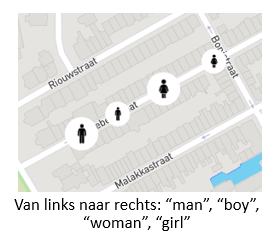
\includegraphics[trim={0 0.3cm 0 0}, clip,scale=1]{sim2.png}}
        \caption{Visualisatie verschillende types}
        \label{02}
    \end{figure}
    
\end{itemize}
\newpage
\textbf{Agenda's}
\begin{itemize}
    \setlength\itemsep{1.5em}
    \item Het \textbf{shopgedrag} is realistischer gemaakt. Hierbij gaat de agent naar een willekeurig aantal willekeurige winkels in de omgeving. In elke winkel blijft de agent 15 tot 30 minuten. In figuur \ref{03} is een simulatie van het shopgedrag te zien.
        \emph{ 
            \begin{enumerate}
                \item Er wordt een willekeurig getal tussen 2 en 5 genomen. Dit getal staat voor het aantal winkels waar de agent naartoe gaat.
                \item Er wordt een willekeurige winkel binnen een straal van 500m van de agent gekozen. De functie die een willekeurige locatie van een bepaald type (zoals winkel) binnen een gebied selecteert bestaat al.
                \item Aan de agenda van de agent wordt toegevoegd dat deze naar de geselecteerde winkel loopt.
                \item Er wordt een willekeurige tijdsduur tussen de 15 en 30 minuten toegevoegd. Aan de agenda van de agent wordt toegevoegd dat deze voor de geselecteerde tijdsduur op zijn locatie blijft staan. Het stilstaan in een winkel wordt gezien als winkelen.
                \item Stappen 2, 3 en 4 worden in een for-loop voor elke winkel herhaald.
            \end{enumerate}
        }
     \begin{figure}[H]
        \centering
            \fbox{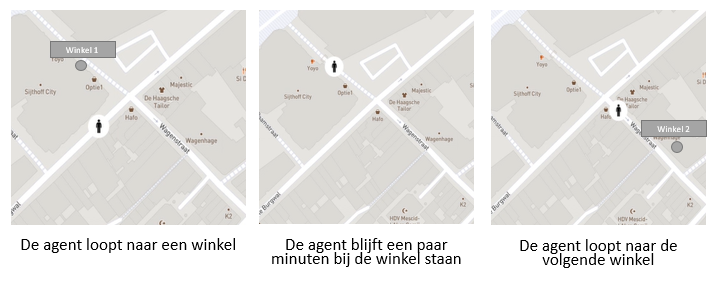
\includegraphics[trim={0 0.2cm 0 0}, clip,scale=0.9]{sim3.png}}
        \caption{Shopgedrag}
        \label{03}
    \end{figure}
    
    \item Er is een agenda toegevoegd waarbij een agent \textbf{rondhangt in een specifiek gebied}. Met rondhangen wordt bedoeld dat de agent naar verschillende plekken in een gebied loopt en stil staat. De agenda is met name toegevoegd om het gedrag van toeristen in de simulatie te kunnen verwerken.
        \emph{ 
            \begin{enumerate}
                \item Er wordt een willekeurige locatie binnen een gebied geselecteerd. Dit wordt gedaan door met behulp van een functie die lijkt op de functie die bij het shopgedrag winkels selecteert. In plaats van de locatie van de agent wordt het middelpunt van het gebied meegegeven. Als maximale afstand wordt de straal van het gebied geselecteerd. De functie selecteert dus een willekeurige locatie waarvan de afstand tussen de locatie en het middelpunt van het gebied gelijk aan of kleiner dan de straal van het gebied is.
                \item Aan de agenda van de agent wordt toegevoegd dat deze naar de gekozen locatie gaat.
                \item Er wordt een willekeurig getal tussen 10 en 20 genomen. Dit getal staat voor het aantal locaties waar de agent naartoe gaat.
                \item Er wordt een willekeurige locatie binnen het gebied gekozen. Dit gaat op dezelfde manier als in stap 1.
                \item Aan de agenda van de agent wordt toegevoegd dat deze naar de geselecteerde locatie loopt.
                \item Er wordt een willekeurige tijdsduur tussen de 0 en 15 minuten toegevoegd. Aan de agenda van de agent wordt toegevoegd dat deze voor de geselecteerde tijdsduur op zijn locatie blijft staan.
                \item Stappen 4, 5 en 6 worden in een for-loop voor elke locatie herhaald.
            \end{enumerate}
        }
    Een simulatie van een agent die rond hangt in een park is in figuur \ref{04} te zien.
     \begin{figure}[H]
        \centering
            \fbox{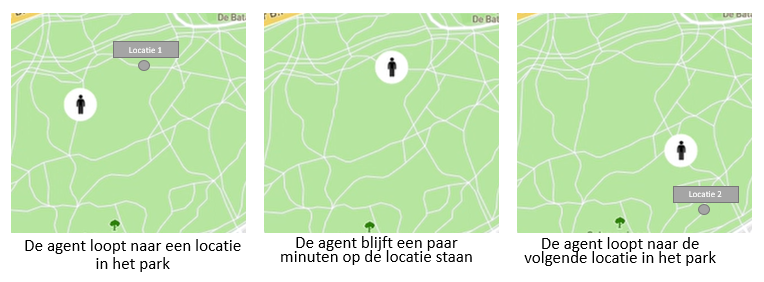
\includegraphics[trim={0 0.3cm 0 0}, clip,scale=0.85]{sim4.png}}
        \caption{Rondhangen in een park}
        \label{04}
    \end{figure}
    
\end{itemize}
\textbf{Overig}
\begin{itemize}
    \setlength\itemsep{1.5em}
    \item Een agent type ``group'' is toegevoegd die een \textbf{groep} representeert toegevoegd: 
        \begin{list}{$\circ$}{}  
            \item In plaats van een icoon is in de visualisatie in de cirkel een getal te zien die aangeeft hoeveel mensen in de groep zitten. 
            \item Als op de groep wordt geklikt wordt een lijst zichtbaar met de id’s van de agents die in de groep zitten.
            \item Wanneer een agent in een groep zitten wordt deze in de visualisatie onzichtbaar. Alleen de groep is dus op dat moment gevisualiseerd en niet zowel de groep als de agents die erin zitten. Dit is gedaan om de visualisatie overzichtelijk te houden.
            \item Wanneer een groep leeg is wordt deze in de visualisatie onzichtbaar. Er zijn dus alleen groepen zichtbaar die daadwerkelijk agents bevatten.
            \item De groep kan de taak krijgen om een of meerdere agents "los te laten". Hiermee wordt bedoeld dat de agents de groep verlaten en weer hun eigen agenda volgen. Dit is in figuur \ref{05} te zien. 
            \item Terwijl de agents in een groep zitten worden hun agenda's gepauzeerd en volgen ze de agenda van de groep.
            \item Er kunnen ook niet bestaande agents in een groep zitten. Wanneer bijvoorbeeld wordt meegegeven dat een groep uit 5000 agents bestaat worden 5000 id's gegenereerd. Bij deze id's horen dan nog geen agents, dus geen eigenschappen en agenda's. Wanneer bij het loslaten van agents een id wordt geselecteerd van een niet-bestaande agent wordt bij het loslaten een nieuwe agent gegenereerd met het geselecteerde id. Deze agent krijgt op dit moment eigenschappen en een agenda.\\ Op deze manier kunnen grote groepen in een simulatie worden toegevoegd zonder in de knoop te raken met het maximale aantal gegenereerde agents dat de omgeving aankan.
        \end{list}
    \begin{figure}[H]
        \centering
            \fbox{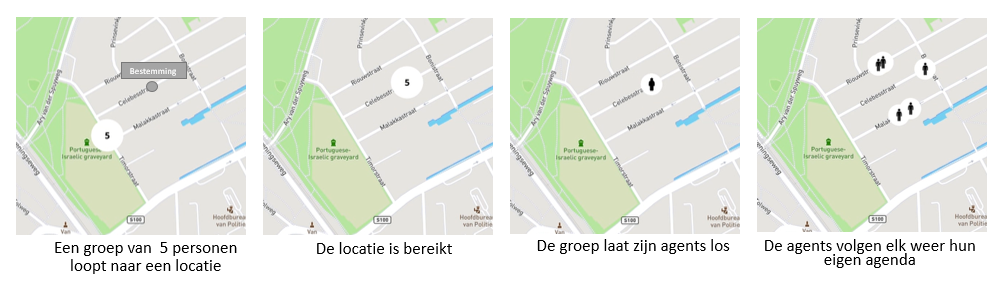
\includegraphics[trim={0 0.3cm 0 0}, clip,scale=0.65]{sim5.png}}
        \caption{Agent type groep}
        \label{05}
    \end{figure}
    
    \item Het gebruik van \textbf{voertuigen} is uitgebreid:
        \begin{list}{$\circ$}{}  
            \item Agents kunnen zowel een auto als een fiets bezitten. In de visualisatie was een icoon voor de auto’s al aanwezig, die van fietsen is toegevoegd. Deze icoons zijn te zien in figuur \ref{06}
            \item De cirkel die het voertuig representeert heeft dezelfde kleur als de bestuurder. Als de bestuurder dus bijvoorbeeld bij team ROOD hoort krijgt de cirkel van de auto een rode kleur.
            \item Wanneer een agent een afstand groter dan 7,5 km af moet leggen wordt gekeken of de agent een auto bezit en of deze zich in de buurt van de agent bevindt. Als dit beide het geval is gaat de agent met de auto naar de bestemming.
            \item Wanneer de afstand die de agent af moet leggen groter is dan 1 km en de agent neemt niet de auto (dus de afstand is korter dan of gelijk aan 7,5 km, de agent bezit geen auto of de auto van de agent staat te ver weg) wordt gekeken of de agent een fiets bezit. Als dit het geval is en de fiets staat in de buurt van de agent, dan gaat de agent op de fiets naar de bestemming.
            \item Wanneer een voertuig niet gebruikt wordt deze onzichtbaar gemaakt in de visualisatie. Dit bevordert de overzichtelijkheid van de simulatie. Het voertuig wordt zichtbaar zodra een agent naar het voertuig begint te lopen om vervolgens met het voertuig zijn bestemming te bereiken.
            \item Wanneer een agent in een voertuig zit is de agent niet zichtbaar. Als een agent bijvoorbeeld in een auto zit is in de visualisatie alleen de auto zichtbaar en niet zowel de auto als de agent.
            \item Als op een voertuig wordt geklikt in de visualisatie wordt een lijst zichtbaar van alle agents die zich in het voertuig bevinden.
        \end{list}
        In figuur \ref{07} is de visualisatie hiervan te zien.
    \begin{figure}[H]
        \centering
            \fbox{
            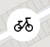
\includegraphics[trim={0 0 0 0}, clip,scale=2]{sim6.png}
            
\includegraphics[trim={0 0 0 0.1cm}, clip,scale=2]{sim6.2.png}
            }
        \caption{icoon fiets en auto}
        \label{06}
    \end{figure}
    
    \begin{figure}[H]
        \centering
            \fbox{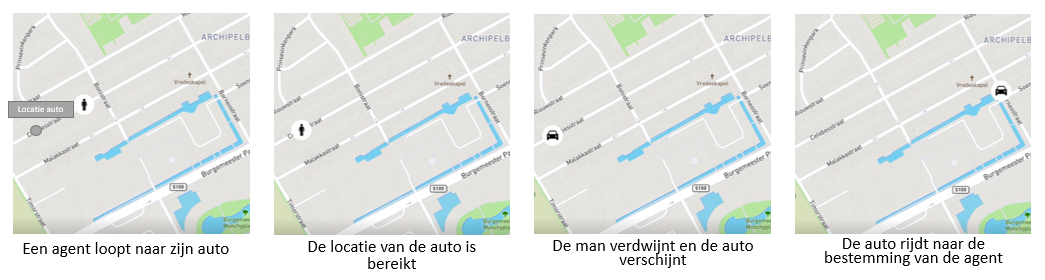
\includegraphics[trim={0 0.3cm 0 0}, clip,scale=0.65]{sim7.png}}
        \caption{Gebruik voertuig}
        \label{07}
    \end{figure}
    
    \item Er is een optie toegevoegd om een \textbf{aankomsttijd} aan een taak mee te geven. Dit wordt gebruikt voor taken waarbij een agent naar een locatie gaat. De agent bereikt de locatie dan op het meegegeven tijdstip. Zo kunnen bijvoorbeeld meerdere agents van verschillende startlocaties tegelijk bij hun bestemming arriveren, zoals in figuur \ref{08} te zien is. 
        \emph{ 
            \begin{enumerate}
                \item De route die de agent neemt om de locatie te bereiken wordt bepaald. Hierbij wordt rekening gehouden met het vervoersmiddel dat de agent neemt. Als de agent met de auto naar de locatie gaat wordt dus een autoroute gekozen.
                \item De snelheid waarmee de agent voortbeweegt wordt bepaald.
                \item Aan de hand van de route en de snelheid wordt de totale duur van de route berekend. Door deze duur van de eindtijd af te trekken wordt de starttijd van het plan berekend. Deze route wordt bepaald met behulp van de gebruikte OSRM routing service.
                \item De agent wacht tot de starttijd is bereikt met het starten van het plan.
            \end{enumerate}
        }
        
    \begin{figure}[H]
        \centering
            \fbox{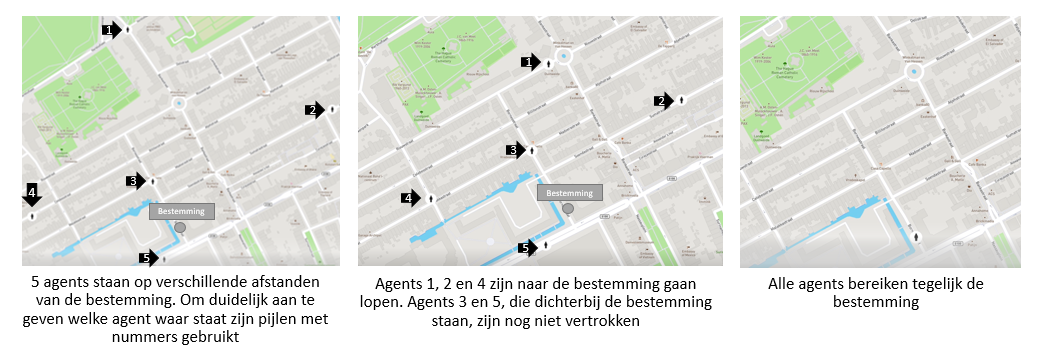
\includegraphics[trim={0 0.3cm 0 0}, clip,scale=0.65]{sim7.1.png}}
        \caption{Aankomsttijd.}
        \label{08}
    \end{figure}
    
\end{itemize}
\subsubsection{Uitbreidingen voor dreigingsscenario's} \label{dreig uitbr}
\textbf{Eigenschappen} \\
De volgende eigenschappen zijn aan agents toegevoegd:
\begin{itemize}
    \setlength\itemsep{1.5em}
    \item Paniek factor: \\
    De paniek factor is een factor met een waarde van minimaal 0 en maximaal 100. Een waarde van 0 geeft aan dat er geen paniek is en een waarde van 100 geeft de maximale hoeveelheid paniek aan.
    \\De paniekfactor wordt met name gebruikt bij het berekenen van de snelheid van een groep, zoals in hoofdstuk \ref{gedrag} staat beschreven, en om het duidelijk te maken dat er sprake is van vluchtgedrag. 
    \\Wanneer een dreiging plaatsvindt verhoogt de paniekfactor met een getal dat aan de dreiging wordt toegekend. 
    \item Vertragingsfactor: \\
    Er kunnen gevallen ontstaan waarin een agent wordt vertraagd door zijn omgeving. Een voorbeeld hiervan is dat een agent minder goed kan zien wanneer er zichtbaar gas is losgelaten. 
    \\ De vertragingsfactor heeft een waarde van 0 wanneer er geen vertraging plaats vindt. Bij een maximale vertraging heeft deze factor een waarde van 100. Wanneer een situatie plaatsvindt die voor vertraging zorgt wordt de vertragingsfactor van een agent verhoogt met een waarde die aan de situatie wordt toegekend.
    \\Wanneer in de visualisatie op de agent wordt geklikt wordt ook de oorzaak van de vertraging zichtbaar.
    \\De snelheid van de agent is gelijk aan de snelheid die de agent zonder vertraging zou hebben gedeeld door een waarde van ($1 + \text{vertragingsfactor}/50$).
    \item Health: \\
    Health is een de eigenschap die aangeeft of een agent gewond is. Wanneer een agent niet gewond is is de waarde van health gelijk aan 100. Als de waarde gelijk is aan 0 is de agent dood. Dode agents krijgen in de visualisatie een donkerdere kleur en bewegen niet meer. 
    \begin{list}{$\circ$}{}
        \item Wanneer health een waarde heeft die lager is dan 30, maar hoger dan of gelijk aan 20, wordt de snelheid van de agent gedeeld door 1,5. De agent loopt dus langzamer als deze erg gewond is.
        \item Bij een waarde lager dan 20 wordt de snelheid van de agent gehalveerd.
        \item Als de waarde lager is dan 10 is de agent zodanig verwond dat deze niet meer kan lopen. De agent staat dus stil en de snelheid is gelijk aan 0.
    \end{list}
    \item Equipment: \\
    Deze eigenschap bevat informatie over de wapens die de agent bij zich draagt. Deze informatie beschrijft het soort wapen, de schade die het wapen creëert en het aantal keer dat het wapen kan worden gebruikt. Met dit laatste wordt bijvoorbeeld het aantal kogels van een handvuurwapen bedoeld.
    \\De schade die het wapen kan creëren wordt gegeven in de vorm van een getal. Dit getal wordt "damage level" \ genoemd en heeft een waarde van minimaal 1 en maximaal 5.
\end{itemize}
\textbf{Team ROOD}
\begin{itemize}
    \setlength\itemsep{1.5em}
    \item Een agent type \textbf{``drone''} is toegevoegd. 
        \begin{list}{$\circ$}{}
            \item Deze agents kunnen losse drones of een zwerm drones representeren.
            \item In de visualisatie is de agent te zien als een cirkel met in het midden een icoon van een drone. Als er sprake is van een zwerm drones is rechtsboven het icoon een getal zichtbaar dat aangeeft hoeveel drones in de zwerm zitten. De cirkel krijgt de kleur die hoort bij het team dat aan de agent is toegekend. Dit zal meestal rood zijn.
            \item De drones vliegen in een rechte lijn naar hun bestemming. Er wordt vanuit gegaan dat de drones hoog genoeg vliegen om geen rekening te hoeven houden met gebouwen. Bij het bepalen van de route van een drone wordt dan ook geen gebruik gemaakt van de OSRM service.
        \end{list}
    Het gebruik van drones is getoond in figuur \ref{09}.
    \begin{figure}[H]
        \centering
            \fbox{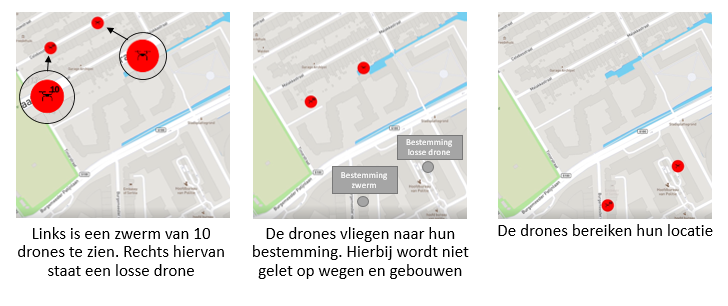
\includegraphics[trim={0 0.3cm 0 0}, clip,scale=0.8]{sim8.png}}
        \caption{Drones}
        \label{09}
    \end{figure}
    
    \item Er is een taak \textbf{"Play Message"} toegevoegd. Deze taak kan aan de agenda van een rode agent worden toegevoegd. Hier wordt mee bedoeld dat een dreigende boodschap wordt afgespeeld. Er wordt dus niemand direct aangevallen, maar er ontstaat wel paniek.
        \begin{list}{$\circ$}{}
            \item Zodra het bericht wordt afgespeeld worden de agenda's van agents die tot team WIT behoren en zich binnen een straal van 200 meter van de agent die het bericht afspeelt bevinden zodanig aangepast dat ze weg rennen van de locatie waar het bericht wordt afgespeeld. Het weg rennen wordt later dit hoofdstuk verder toegelicht.
            \item De paniek factor van de agents van team WIT die op het bericht reageren wordt verhoogd met 10.
        \end{list}
    \item Agents van team ROOD kunnen \textbf{van een witte naar een rode groep} lopen. Dit is toegevoegd voor een scenario waar een aantal agents van team ROOD tot een groep behoren die als team WIT wordt gezien. Hier komt een rode groep langs die bijvoorbeeld aan het rellen is. De agents uit het witte team zien dat en de agents die tot team ROOD behoren verlaten de witte groep en voegen zich bij de rode groep en nemen deel aan de dreiging. Het wisselen van groep is in figuur \ref{10} zichtbaar.
        \emph{ 
            \begin{enumerate}
                \item Eerst wordt een lijst gemaakt van alle agents van team ROOD die in de witte groep zitten.
                \item Één van deze agents wordt geselecteerd en losgelaten uit de groep.
                \item De losgelaten agent krijgt als eerste agenda-punt de taak om zich bij een rode groep te voegen. Hierbij wordt gezocht naar rode groepen binnen een straal van 1km naar de agent. 
                \item Als dit meerdere groepen zijn wordt hier willekeurig één van gekozen en hier loopt de agent naartoe. In het geval van één rode groep loopt de agent naar deze groep.
                \item Zodra de agent de locatie van de rode groep heeft bereikt voegt de agent zich bij de groep.
                \item Stap 2 t/m 5 voor de volgende agent van team ROOD uitgevoerd, tot alle agents van team ROOD van de witte groep hebben verlaten. 
            \end{enumerate}
        }
        
    \begin{figure}[H]
        \centering
            \fbox{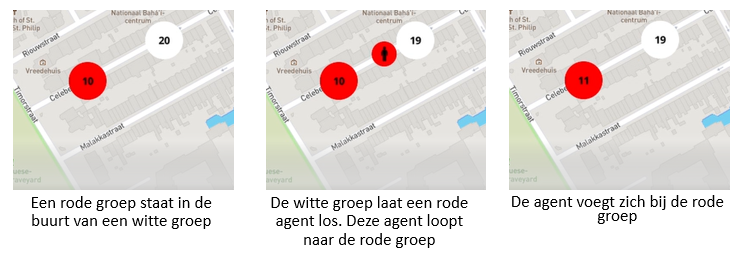
\includegraphics[trim={0 0.3cm 0 0}, clip,scale=0.9]{sim9.png}}
        \caption{Wisselen van witte naar rode groep}
        \label{10}
    \end{figure}
    
    \item Er is een agenda toegevoegd waar een agent een \textbf{winkel berooft}, zoals te zien is in figuur \ref{11}: 
       \emph{ 
            \begin{enumerate}
                \item De agent gaat naar de winkel die hij zal beroven.
                \item De agent blijft 10 minuten in de winkel.
                \item Hierna rent de agent weg uit de winkel. De snelheid van de agent is tijdens het wegrennen verdubbeld.
            \end{enumerate}
        }
        \begin{figure}[H]
        \centering
            \fbox{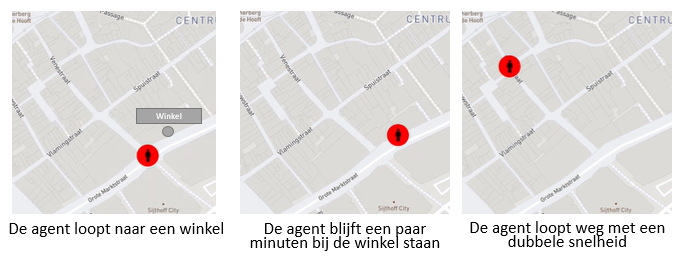
\includegraphics[trim={0 0.3cm 0 0}, clip,scale=0.9]{sim10.png}}
        \caption{Winkel beroven}
        \label{11}
    \end{figure}
    \newpage
    \item Een agent kan een \textbf{object} achterlaten:
        \begin{list}{$\circ$}{}
            \item Het object wordt als een aparte agent aangemaakt. Er is een type agent voor een bom, een type voor gas en een type voor een overig object.
            \item Het object wordt op dezelfde manier meegenomen als een persoon door een groep wordt meegenomen. Het object heeft dus zolang de agent hem vast heeft geen agenda en is niet zichtbaar.
            \item Zodra de agent het object loslaat verschijnt het object. Een overig object is afgebeeld als een cirkel zonder icoon. Een bom krijgt een icoon van een bom en gas krijgt een icoon van een wolk om aan te duiden dat het om gas gaat. De cirkel van een gas-object is groter dan die van een gewone agent en een beetje doorzichtig. 
            \item Een overig object blijft staan op de plek waar deze is achtergelaten en krijgt verder geen agenda.
            \item Een bom blijft na het achterlaten 10 minuten tot een kwartier staan. Hierna ontploft de bom. Bij het ontploffen gaan alle agents binnen een straal van 5 meter dood. De overige agents binnen een straal van 15 meter van de bom raken gewond. Bij de gewonden verminderd de eigenschap "health" \ met een willekeurige waarde tussen 50 en 100. Witte agents binnen een straal van 300 meter rennen weg met een paniek factor van 100.
            \item Gas blijft een duur van 15 tot 30 minuten op de plek waar het is achtergelaten. Hierna verdwijnt het. Er wordt uitgegaan van gas dat niet giftig is, het wordt alleen gebruikt om paniek te creëren. Witte agents binnen een straal van 300 meter rennen weg met een paniek factor van 50 en een vertragingsfactor van 30.
        \end{list}
    Figuur \ref{12} toont de verschillende objecten. Een voorbeeld van een simulatie waar een agent een bom achterlaat is zichtbaar in figuur \ref{13}   
        \begin{figure}[H]
        \centering
            \fbox{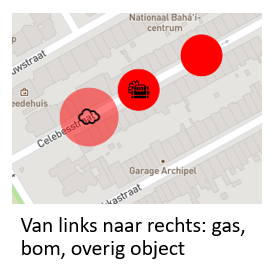
\includegraphics[trim={0 0.3cm 0 0}, clip,scale=0.8]{sim13.png}}
        \caption{Objecten}
        \label{12}
    \end{figure}
    \begin{figure}[H]
        \centering
            \fbox{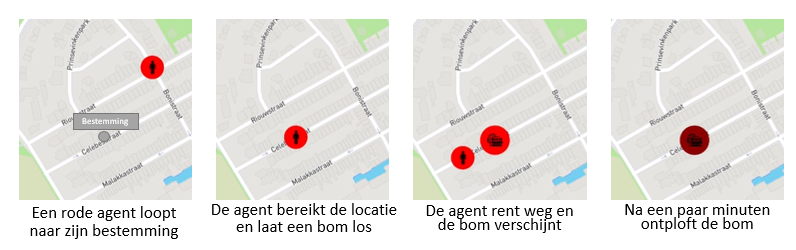
\includegraphics[trim={0 0.3cm 0 0}, clip,scale=0.8]{sim11.png}}
        \caption{Achterlaten object}
        \label{13}
    \end{figure}
    
    \item Er is een agenda genoemd \textbf{"Chaos"} toegevoegd. Hier hebben de agents van team ROOD het doel om zoveel mogelijk slachtoffers te creëren.
              \emph{ 
            \begin{enumerate}
                \item Om chaos in deze vorm te kunnen creëren moet agent van team ROOD wapens bij zich dragen. Dit wordt aan de agent toegekend met de eigenschap ``equipment''.
                \item Indien een gebied wordt gegeven waarin de agent chaos moet creëren wordt een willekeurige locatie geselecteerd binnen dit gegeven gebied. Dit gaat op dezelfde manier als bij het rondhangen in een specifiek gebied in paragraaf \ref{alg uitbr}. Wanneer geen gebied is meegegeven wordt een willekeurige locatie binnen een straal van 50 meter van de agent geselecteerd.
                \item De agent loopt naar de locatie. Terwijl de agent naar de locatie loopt voert hij een aanval uit. Alle witte agents die zich binnen een straal van 300 meter van de aanvaller bevinden rennen weg. De paniekfactor van deze agents is gelijk aan 100.
                \item Bij het uitvoeren van een aanval wordt een willekeurig wapen gekozen. Dit wapen wordt geselecteerd uit de eigenschap ``equipment''.
                \begin{list}{$\circ$}{}
                    \item Als het geselecteerde wapen een handvuurwapen is wordt een willekeurige agent binnen een straal van 200 meter van de aanvaller gekozen. De schade is gelijk aan het damage level van het wapen vermenigvuldigd met een willekeurig getal tussen 10 en 20. Deze schade wordt van de eigenschap "health" \ van de agent af getrokken. Als de kogels van het wapen op zijn wordt het wapen met zijn eigenschappen uit ``equipment'' verwijderd. 
                    \item Als het geselecteerde wapen een handgranaat is wordt een locatie binnen een straal van 100 meter van de agent gekozen. Deze locatie is minimaal 20 meter van de agent verwijderd, zodat de agent zelf niet door de handgranaat gewond raakt. Alle agents binnen een straal van 5 meter van de gekozen locatie gaan dood. De overige agents binnen een straal van 15 meter van de locatie raken gewond. Bij de gewonden verminderd de eigenschap "health" \ met een willekeurige waarde tussen 50 en 100. Als de handgranaten op zijn wordt het wapen met zijn eigenschappen uit ``equipment'' verwijderd.
                \end{list}
                \item Stappen 2, 3 en 4 worden herhaald zolang de agent van team ROOD nog wapens heeft en niet te gewond is. Zodra de waarde van de eigenschap "health" \ van de agent 30 of lager is wordt de agent als te gewond gezien.
                \item De agent kan een eigenschap krijgen die aangeeft dat hij een bomvest draagt. Als dit het geval is wordt zodra de agent te gewond is of zijn wapens op zijn gekeken of binnen een straal van 15 meter van de agent een groep aanwezig is. Als dit het geval is loopt de aanvaller naar de groep toe.
                \item Als er geen groep in de buurt van de agent staat wordt gekeken of een losse agent binnen een straal van 15 meter van de agent staat. Als deze losse agent er is loopt de aanvaller hier naartoe. Als er geen agent dichtbij genoeg staan blijft de agent van team ROOD op zijn plek.
                \item De agent laat zijn bomvest ontploffen. Alle agents binnen een straal van 5 meter van de agent, waaronder de agent zelf gaan dood. De overige agents binnen een straal van 15 meter van de agent raken gewond. Bij de gewonden verminderd de eigenschap "health" \ met een willekeurige waarde tussen 50 en 100.
            \end{enumerate}
        }  
    Deze agenda is in figuur \ref{14} te zien.           
    \begin{figure}[H]
        \centering
            \fbox{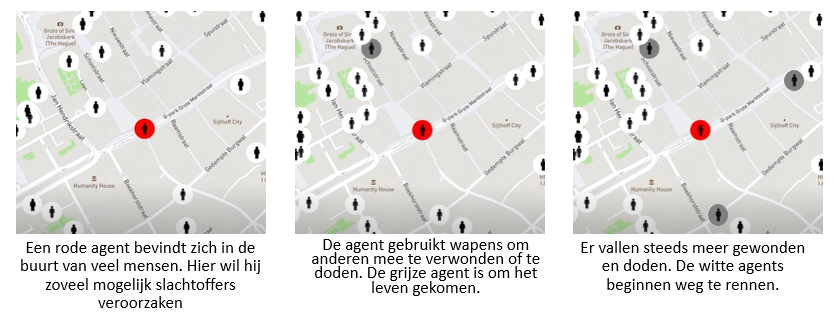
\includegraphics[trim={0 0.3cm 0 0}, clip,scale=0.8]{sim13.1.png}}
        \caption{Chaos}
        \label{14}
    \end{figure}
    
\end{itemize}

\textbf{Vluchtgedrag team WIT}
\begin{itemize}
    \setlength\itemsep{1.5em}
    \item Bij de meeste dreigingen is de reactie van team WIT \textbf{wegrennen}. Deze reactie is aan de simulatie-omgeving toegevoegd. 
        \emph{ 
            \begin{enumerate}
                \item De locatie van de dreiging wordt aan de agents meegegeven. Het is ook mogelijk om aan te geven tot welke afstand van de dreiging de agents weg moeten rennen. Als deze afstand niet wordt meegegeven wordt een afstand van 500 meter aangehouden. 
                \item De helling van de lijn tussen de locatie van de agent en de locatie van de dreiging wordt berekend. Dit wordt gedaan zodat de agent in tegengestelde richting van de dreiging rent. De helling wordt berekend door het verschil in breedtegraden van de locaties te delen door het verschil in lengtegraden.
                \item De afstand, die in stap 1 beschreven staat, wordt omgezet naar graden. Dit wordt gedaan door de afstand in meters te delen door het getal 111139 (de factor waarmee graden naar meters kunnen worden geconverteerd).
                \item Het verschil in lengtegraden dat nodig is om de gewenste afstand af te leggen over de lijn tussen de agent en de dreiging wordt berekend aan de hand van de volgende formule: $\text{verschilLengtegraden} = \sqrt{(\text{afstandInGraden}^2) / (1 + \text{helling}^2)}$. Deze formule is afgeleid van de stelling van Pythagoras ($\text{a}^2 + \text{b}^2 = \text{c}^2 $) en de standaard functie van een lijn ($y = a \cdot x + b$). 
                \item Als de lengtegraad van de locatie van de agent kleiner is dan die van de locatie van de dreiging wordt het berekende nodige verschil in lengtegraden vermenigvuldigd met -1. 
                \item Het berekende nodige verschil in lengtegraden wordt bij de lengtegraad van de locatie van de dreiging opgeteld. Het nodige verschil in lengtegraden vermenigvuldigd met de berekende helling wordt bij de breedtegraad van de locatie van de dreiging opgeteld. Deze lengte- en breedtegraad vormen de coördinaten van het punt dat de gewenste afstand verwijderd is van de dreiging en zich in tegengestelde richting van de dreiging ten opzichte van de agent bevindt.
                \item Om de eindlocatie van de agent iets realistischer te maken wordt een willekeurige locatie binnen een straal van 10 meter om de berekende locatie heen gekozen. Dit is de eindlocatie waar de agent naartoe rent. Door een locatie binnen een straal van 10 meter te kiezen is de eindlocatie iets willekeuriger, maar rent de agent toch altijd in tegengestelde richting van het gevaar.
                \item De agent gaat naar de eindlocatie. De snelheid van de agent is hier het dubbele van zijn normale snelheid.
            \end{enumerate}
        }
     In figuur \ref{15} is een simulatie te zien waar een agent van team WIT weg rent van een bom.         
    \begin{figure}[H]
        \centering
            \fbox{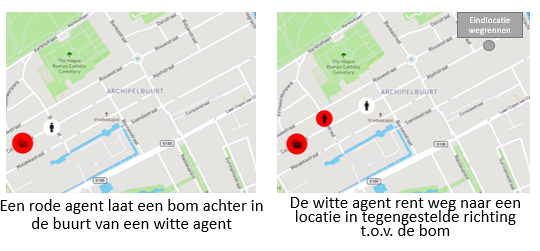
\includegraphics[trim={0 0.3cm 0 0}, clip,scale=0.8]{sim14.png}}
        \caption{Wegrennen}
        \label{15}
    \end{figure}
    
    \item In een dreigingsscenario raken mensen binnen een massa vluchtende mensen gewond. Dit gebeurt bijvoorbeeld doordat iemand valt en anderen over deze persoon heen rennen. Door de manier waarop grote groepen in de omgeving zijn gesimuleerd kan niet worden bepaald wanneer iemand binnen een groep over iemand anders binnen dezelfde groep heen rent. Toch is het gewenst om dit \textbf{vluchtgedrag van groepen} in de simulatie te verwerken. Dit is op de volgende manier gedaan:
        \emph{ 
            \begin{enumerate}
                \item Een groep toont vluchtgedrag als de paniekfactor een waarde heeft die groter is dan 0 en de groep aan het rennen is.
                \item De kans dat een groep gewonden achterlaat is afhankelijk van de grootte van de groep, de paniekfactor en de kwetsbaarheid van een groep. In een groep ouderen zullen meer gewonden vallen dan in een groep jongvolwassenen. De kwetsbaarheid van een groep wordt gemeten aan de hand van een eigenschap genaamd "vulnerability". Wanneer een groep niet kwetsbaar is krijgt deze factor een waarde van 0. Bij een extreem kwetsbare groep heeft deze eigenschap een waarde van 100.\\
                De kans dat een groep gewonden achterlaat wordt berekend met de volgende formule: $\text{kans} = (\text{paniekfactor}/200 + \text{vulnerability}/200) \cdot \text{aantalMensenInGroep} \cdot 0.01$ 
                \item Een willekeurig getal tussen 0 en 100 wordt gekozen. Als dit getal lager is dan de kans dat een gewond persoon wordt achtergelaten worden 1 tot 3 agents uit de groep losgelaten. Het is willekeurig of het om 1, 2 of 3 agents gaat.
                \item De eigenschap "health" \ van de losgelaten agents krijgt een willekeurige waarde tussen 0 en 30. Op deze manier wordt aangegeven dat de agent zodanig gewond is dat deze achterblijft en niet meer met de groep meegaat.
                \item Als de waarde van "health" \ hoog genoeg is om nog te kunnen lopen, dus 10 of hoger, vlucht de agent na een wachttijd van drie minuten verder.
                \item Als de losgelaten agent tot een subgroep behoort, zoals een familie, wordt gekeken of de andere leden van deze subgroep nog in de groep aanwezig zijn. Als dit het geval is worden deze agents ook losgelaten. Dit wordt gedaan met het idee dat een ouder bij zijn gewonde kind zal blijven.
            \end{enumerate}
        }
    In figuur \ref{16} is te zien hoe een groep tijdens het vluchten een gewonde agent achterlaat.
    \begin{figure}[H]
        \centering
            \fbox{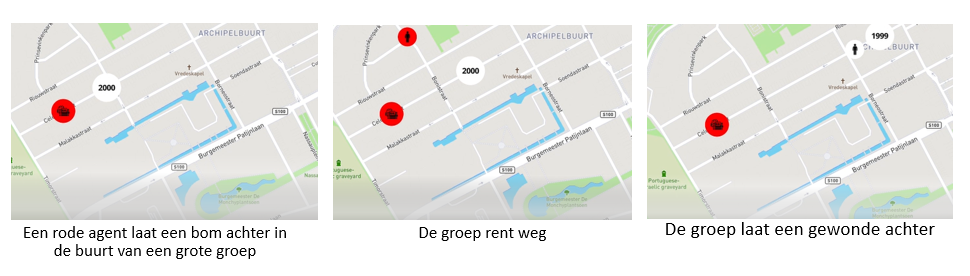
\includegraphics[trim={0 0.3cm 0 0}, clip,scale=0.65]{sim15.png}}
        \caption{Vluchtgedrag groep}
        \label{16}
    \end{figure}
    
    
    \item Voor losse vluchtende agents, dus agents die niet onderdeel zijn van een groep, is het vluchtgedrag als volgt gedefinieerd: 
        \emph{ 
            \begin{list}{$\circ$}{}
                \item Als binnen een radius van 1 meter om de agent heen een groep witte agents staat sluit de agent zich bij deze groep aan.
                \item Als binnen een radius van 1 meter om de agent heen een andere agent staat is er een kans van 30 procent dat er een botsing plaats vindt. In dat geval staat de agent 1 tot 3 minuten stil en neemt de eigenschap health af met een waarde tussen 0 en 15.
            \end{list}
        }

    
\end{itemize}



\newpage
\section{Conclusie} \label{conclusie}
In dit hoofdstuk wordt antwoord gegeven op de hoofdvraag: Hoe kunnen dreigingsscenario's zodanig worden gesimuleerd dat de effecten en acties van betrokkenen in een scenario zichtbaar zijn? \\ \\
In paragrafen \ref{alg uitbr} en \ref{dreig uitbr} staat een opsomming van toevoegingen aan de simulatie-omgeving beschreven. Dit is een lijst van type agents, eigenschappen, acties, reacties en verbeteringen aan de visualisatie van het model. Het gaat om de volgende toevoegingen:
\begin{itemize}
    \item Het zichtbaar en onzichtbaar maken van agents in de visualisatie, zodat alleen agents die op het moment dat ze relevant zijn zichtbaar zijn
    \item Het toekennen van het juiste team aan de agent (WIT, ROOD of BLAUW) en dit aan de hand van een bijhorende kleur verwerken in de visualisatie
    \item Het visualiseren van vrouwen en kinderen
    \item Een type agent voor groepen. De snelheid van een groep wordt bepaald aan de hand berekeningen die in hoofdstuk \ref{gedrag} staan beschreven
    \item Het uitbreiden van het gebruik van vervoersmiddelen aan de hand van de afstand tot de eindbestemming
    \item Een agenda voor realistisch shopgedrag
    \item Een agenda voor het rondhangen in een specifiek gebied
    \item Een aankomsttijd die er bijvoorbeeld voor kan zorgen dat alle betrokkenen tegelijk om hun locatie aankomen
    \item Een paniekfactor en een vertragingsfactor
    \item Een eigenschap die aangeeft of een agent verwond is en hoe ernstig de verwondingen zijn
    \item Een eigenschap die aangeeft of een agent wapens bij zich draagt en informatie over deze wapens geeft
    \item Een type agent voor drones
    \item Een optie om een dreigende geluidsboodschap af te spelen
    \item Een optie om agents van team ROOD een groep van team WIT te verlaten en zich bij een groep van team ROOD te voegen
    \item Een agenda om een winkel te beroven
    \item Een optie om gas dat na een bepaalde tijd verdwijnt, een bom die na een bepaalde tijd ontploft, of een overig object achter te laten
    \item Een agenda waar een agent van team ROOD met behulp van wapens zoveel mogelijk slachtoffers in een gebied creëert.
    \item Agents van team WIT rennen als reactie op bepaalde dreigingen weg van de dreiging
    \item Vluchtende groepen laten, afhankelijk van de grootte van de groep, de aanwezigheid van paniek en de kwetsbaarheid van de groep, slachtoffers achter
    \item Gestorven agents krijgen in de visualisatie een donkerdere kleur
    
\end{itemize}
Het verwerken van deze zaken in de simulatie-omgeving zorgt ervoor dat de betrokkenen in dreigingsscenario's en diens acties en reacties zichtbaar zijn in de visualisatie van de simulatie. De effecten van acties van betrokkenen zijn zichtbaar in de vorm van het verschijnen van een object, een reactie van andere betrokkenen of, in het geval van een gestorven betrokkenen, een donkerdere kleur van de cirkel die de agent visualiseert. 



\newpage
\section{Aanbevelingen} \label{advies}
In hoofdstuk \ref{Heigenschappen} staat een onderzoek naar eigenschappen van betrokkenen in dreigingsscenario's beschreven. De resultaten hiervan zijn nog niet in het simulatiemodel verwerkt. Mijn advies is om bij het verder uitbreiden en verbeteren van de simulatie-omgeving de berekende verhoudingen in de omgeving te verwerken. Dit zorgt voor representatieve eigenschappen van personen in een scenario.\\ 
Ook kan onderzoek worden gedaan naar de invloed van deze eigenschappen op de effectiviteit van acties van team BLAUW. De simulatie-omgeving wordt uiteindelijk gebruikt om de effectiviteit van acties van de politie en KMar te evalueren. Uit het statistisch onderzoek is gebleken dat de groep mensen die geweld toont tegen te politie voornamelijk uit mannen bestaat. Er kan worden onderzocht of de oorzaak van deze verhouding is dat mannen anders tegen acties van de politie reageren van vrouwen, of dat mannen vaker in contact komen met de politie waardoor ze zich vaker in een situatie bevinden waar geweld kan worden getoond.
\\ \\
Momenteel bestaat een groot deel van de simulatie-omgeving uit aannames. Een voorbeeld hiervan is de afstand tussen personen in een groep op basis van de grootte van de groep en de paniekfactor. Helaas is het tijdens het onderzoek met de beschikbare tijd en literatuur niet mogelijk geweest om te bepalen of deze aannames het gedrag realistisch weergeeft. Het gaat met name om de volgende aannames:
\begin{itemize}
    \item De gemiddelde afstand tussen mensen in een groep op basis van de groepsgrootte
    \item De invloed van paniek op de afstand tussen mensen in een groep
    \item De invloed van de vertraging die in een aantal scenario's wordt veroorzaakt op de snelheid van mensen
    \item Binnen welke straal van de locatie van de dreiging mensen op de dreiging reageren
    \item De afstand die mensen bij een dreiging afleggen tijdens het wegrennen tot ze zich veilig genoeg voelen om niet meer te rennen
    \item De invloed van de grootte van een groep, de paniekfactor en de kwetsbaarheid van een groep op het achterlaten van gewonden
\end{itemize}
Ik adviseer TNO om hier uitgebreider onderzoek naar te doen. Wanneer deze zaken niet op basis van aannames, maar op basis van een uitgebreid onderzoek worden verwerkt is de simulatie significant realistischer. 
\\ \\
Momenteel worden in de simulaties gebouwen voor een groot deel genegeerd. De OSRM service zorgt ervoor dat mensen niet door gebouwen heen lopen, maar bij het willekeurig selecteren van een slachtoffer of het bepalen welke agents op een situatie reageren wordt geen rekening gehouden met gebouwen. In een werkelijke situatie zouden gebouwen het zicht van mensen belemmeren en wordt niet gemakkelijk met bijvoorbeeld een handvuurwapen door een gebouw heen geschoten. Mijn advies is om bij verdere uitbreiding van de simulatie-omgeving een manier te zoeken om de invloed van gebouwen in het model te kunnen verwerken. 


\newpage
\begin{appendices}
\section{Literatuurlijst}
\subsection{Gevolgde cursussen}
\begin{itemize}
    \item \emph{CSS Tutorial: Learn CSS For Free}. Codecademy. https://www.codecademy.com/learn/learn-css
    \item \emph{HTML Tutorial: Learn HTML For Free}. Codecademy. https://www.codecademy.com/learn/learn-html
    \item \emph{Learn TypeScript}. Codecademy. https://www.codecademy.com/learn/learn-typescript
\end{itemize}
\subsection{Methode}
\begin{itemize}
    \item Boersma, M. (2021). Domain-Specific Languages Made Easy. New York, Verenigde Staten: Manning Publications.
    \item Wikipedia-bijdragers. (2020, 24 maart). Agent-gebaseerd model. Geraadpleegd van https://nl.wikipedia.org/wiki/Agent-gebaseerd\_model
    \item Wikipedia contributors. (2021, 13 april). Entity component system. Geraadpleegd van https://en.wikipedia.org/wiki/Entity\_component\_system
    \item Wikipedia contributors. (2021a, 22 januari). Composition over inheritance. Geraadpleegd van https://en.wikipedia.org/wiki/Composition\_over\_inheritance
\end{itemize}
\subsection{Eigenschappen} \label{bronnencbs}
\begin{itemize}
    \item Centraal Bureau voor de Statistiek. (2021, 26 maart). Kenmerken van verdachten en slachtoffers, 2018-feb 2021. Geraadpleegd van https://www.cbs.nl/nl-nl/maatwerk/2021/12/ \\kenmerken-van-verdachten-en-slachtoffers-2018-feb-2021
    \item Centraal Bureau voor de Statistiek. (2021, 26 maart). Kerncijfers wijken en buurten 2018. Geraadpleegd van https://www.cbs.nl/nl-nl/maatwerk/2018/30/kerncijfers-wijken-en-buurten-2018
    \item Centraal Bureau voor de Statistiek. (2020, 3 september). Geweld en agressie tegen politieambtenaren, 2019. https://www.cbs.nl/nl-nl/maatwerk/2020/36/geweld-en-agressie-tegen-politieambtenaren-2019
\end{itemize}
\subsection{Gedrag} \label{bronnenberekeningen}
\begin{itemize}
    \item Helbing, D., Farkas, I., \& Vicsek, T. (2000). Simulating dynamical features of escape panic. Nature, 407(6803), 487-490
    \item Leijonmarck, E., \& Olergård, T. (2013). Modelling of panicking pedestrians during emergency evacuation.
    \item Thio, N. A. (2019). Pedestrian Crowd Evacuation Under Panic (Doctoral dissertation, The University of Melbourne).
\end{itemize}

\newpage
\section{Tabellen} \label{tabellen}
\begin{table}[H]
    \begin{center}
    {\fontfamily{lmss}\selectfont
        \caption{p-waarden verdachten}
        \resizebox{\textwidth}{!}{\begin{tabular}{|R{2.5cm}||C{1.4cm}||C{1.4cm}|C{1.4cm}|C{1.4cm}||C{1.4cm}|C{1.4cm}|C{1.4cm}|} 
            \hline
            & \multicolumn{7}{c|}{\textbf{p-waarde}}\\ 
            \hline
             & \textbf{Geweld tegen politie} & \multicolumn{3}{c||}{\textbf{Openlijk geweld}} & \multicolumn{3}{c|}{\textbf{Aantasting openbare orde}}\\
            \hline
            \textbf{Categorie} & \textbf{2019} & \textbf{2018} & \textbf{2019} & \textbf{2020} & \textbf{2018} & \textbf{2019} & \textbf{2020} \\
            \hline
            Geslacht &  $2,2\mathrm{e}{-16}$ &   $2,2\mathrm{e}{-16}$ &   $2,2\mathrm{e}{-16}$ &   $2,2\mathrm{e}{-16}$ &   $2,2\mathrm{e}{-16}$ &   $2,2\mathrm{e}{-16}$&   $2,2\mathrm{e}{-16}$\\
            \hline
            Leeftijdsklasse &  $2,2\mathrm{e}{-16}$ &   $2,2\mathrm{e}{-16}$ &   $2,2\mathrm{e}{-16}$ &   $2,2\mathrm{e}{-16}$ &   $2,2\mathrm{e}{-16}$ &   $2,2\mathrm{e}{-16}$&   $2,2\mathrm{e}{-16}$\\
            \hline
            Samenstelling huishouden &  $2,2\mathrm{e}{-16}$ &   $2,2\mathrm{e}{-16}$ &   $2,2\mathrm{e}{-16}$ &   $2,2\mathrm{e}{-16}$ &   $2,2\mathrm{e}{-16}$ &   $2,2\mathrm{e}{-16}$&   $2,2\mathrm{e}{-16}$\\
            \hline
            Migratie achtergrond  &  $2,2\mathrm{e}{-16}$ &   $2,2\mathrm{e}{-16}$ &   $2,2\mathrm{e}{-16}$ &   $2,2\mathrm{e}{-16}$ &   $2,2\mathrm{e}{-16}$ &   $2,2\mathrm{e}{-16}$&   $2,2\mathrm{e}{-16}$\\
            \hline
            Hoogst behaalde opleiding  &  $2,2\mathrm{e}{-16}$ &   $2,2\mathrm{e}{-16}$ &   $2,2\mathrm{e}{-16}$ &   $2,2\mathrm{e}{-16}$ &   $2,2\mathrm{e}{-16}$ &  $2,2\mathrm{e}{-16}$&  $2,2\mathrm{e}{-16}$\\
            \hline
            Inkomenspercentiel & $2,2\mathrm{e}{-16}$ &  $2,2\mathrm{e}{-16}$ &  $2,2\mathrm{e}{-16}$ &  $2,2\mathrm{e}{-16}$ &  $2,2\mathrm{e}{-16}$ &  $2,2\mathrm{e}{-16}$&  $2,2\mathrm{e}{-16}$\\
            \hline
            Stedelijkheidsklasse  & $2,2\mathrm{e}{-16}$ &  $2,2\mathrm{e}{-16}$ &  $2,2\mathrm{e}{-16}$ &  $2,2\mathrm{e}{-16}$ &  $2,2\mathrm{e}{-16}$ &  $2,2\mathrm{e}{-16}$&  $2,2\mathrm{e}{-16}$\\
            \hline
        \end{tabular}}
    \label{res01}
    }
    \end{center}
\end{table}
\begin{table}[H]
    \begin{center}
    \small
        \fontfamily{lmss}\selectfont{
            \caption{Verhoudingen verdachten}
            \begin{tabular}{|R{2.5cm}|R{3.5 cm}||C{2cm}|C{2cm}|C{2cm}|}
                \hline
                \multicolumn{1}{|c|}{\multirow{2}{*}{\textbf{Categorie}}} & \multicolumn{1}{c||}{\multirow{2}{*}{\textbf{Eigenschap}}} & \multicolumn{3}{c|}{\textbf{Percentage} } \\ 
                \cline{3-5}
                &  & Geweld tegen politie & Openlijk geweld & Aantasting openbare orde \\ 
                \hline \hline 
                \rule{0pt}{11pt}
                Geslacht & Man & $89\%$ & $86\%$ & $91\% $ \\
                \cline{2-5}
                \rule{0pt}{11pt}
                & Vrouw & $11\%$ & $14\% $ & $9\%$\\
                \hline 
                \rule{0pt}{11pt}
                Leeftijdsklasse & \textless{}18 & $8\%$ & $35\% $ & $6\%$ \\     
                \cline{2-5} 
                \rule{0pt}{11pt}
                & 18-25 & $28\%$ & $36\%$ & $23\%$ \\
                \cline{2-5} 
                \rule{0pt}{11pt}
                & 25-45 & $47\%$ & $23\%$ & $50\%$\\
                \cline{2-5}
                \rule{0pt}{11pt}
                & $45-65$ & $16\%$ & $23\%$ & $20\%$\\
                \cline{2-5} 
                \rule{0pt}{11pt}
                & \textgreater{}65 & $1\%$ & $1\%$ & $1\%$\\
                \hline 
                \rule{0pt}{5pt}
                Samenstelling huishouden & Eenpersoons huishouden & $36\%$ & $14\%$ & $36\%$ \\ \cline{2-5}
                \rule{0pt}{11pt}
                & (On)gehuwd paar zonder kinderen & $8\%$ & $5\%$ & $7\%$ \\
                \cline{2-5} 
                \rule{0pt}{11pt}
                & (On)gehuwd paar met kinderen & $26\%$ & $47\%$ & $24\%$ \\
                \cline{2-5} 
                \rule{0pt}{11pt}
                & Eenouderhuishouden & $18\%$ & $29\%$ & $14\%$\\
                \cline{2-5}
                \rule{0pt}{11pt}
                & Institutioneel of overig huishouden & $12\%$ & $5\%$ & $19\%$ \\
                \hline 
                \rule{0pt}{11pt}
                Migratie-achtergrond & Geen migratieachtergrond & $50\%$ & $53\%$ & $42\%$ \\  \cline{2-5} 
                \rule{0pt}{11pt}
                & Westerse migratieachtergrond & $11\%$ & $8\%$ & $14\%$ \\
                \cline{2-5} 
                \rule{0pt}{11pt}
                & Niet-westerse migratieachtergrond & $39\%$ & $39\%$ & $44\%$ \\
                \hline
                \rule{0pt}{5pt}
                Hoogst behaalde opleiding & Lager onderwijs & $64\%$ & $73\%$ & $61\%$ \\  \cline{2-5} 
                \rule{0pt}{11pt}
                & Middelbaar onderwijs & $31\%$ & $24\%$ & $32\%$ \\
                \cline{2-5} 
                \rule{0pt}{11pt}
                & Hoger onderwijs & $5\%$ & $3\%$ & $7\%$ \\
                \hline 
                \rule{0pt}{5pt}
                Inkomens-percentiel & 0-25 procent & $54\%$ & $42\%$ & $58\%$ \\
                \cline{2-5} 
                \rule{0pt}{11pt}
                & 25-50 procent & $20\%$ & $23\%$ & $17\%$ \\
                \cline{2-5} 
                \rule{0pt}{11pt}
                & 50-75 procent  & $14\%$ & $19\%$ & $14\%$\\
                \cline{2-5} 
                \rule{0pt}{11pt}
                & 75-100 procent & $12\%$ & $16\%$ & $11\%$ \\ 
                \hline 
                \rule{0pt}{5pt}
                Stedelijkheidsklasse & Zeer stedelijk & $40\%$ & $32\%$ & $43\%$ \\ 
                \cline{2-5} 
                \rule{0pt}{11pt}
                & Sterk stedelijk & $28\%$ & $30\%$ & $26\%$ \\ 
                \cline{2-5} 
                \rule{0pt}{11pt}
                & Matig stedelijk & $13\%$ & $18\%$ & $14\%$ \\ 
                \cline{2-5} 
                \rule{0pt}{11pt}
                & Weinig stedelijk & $10\%$ & $11\%$ & $8\%$ \\
                \cline{2-5} 
                \rule{0pt}{11pt}
                & Niet stedelijk & $9\%$ & $9\%$ & $9\%$ \\
                \hline  
            \end{tabular}
            \label{res02}
            }
    \end{center}
\end{table}

\newpage
\section{Reflectie} \label{reflect}
In dit hoofdstuk wordt gereflecteerd op het verloop van de stage. Hierbij wordt gekeken naar de betrouwbaarheid en representativiteit van de resultaten, naar hoe de uitgevoerde opdracht afwijkt van de oorspronkelijke opdracht en planning die in het Plan van Aanpak waren beschreven en naar het behalen van de doelstelling. Tot slot bevat dit hoofdstuk een terugblik op de opgedane ervaring en de leerzaamheid van de stage.

\subsection{Betrouwbaarheid en representativiteit resultaten}
Tijdens het statistisch onderzoek zijn alle toetsen uitgevoerd op datasets van het CBS. Alle datasets die het CBS publiceert bevatten betrouwbare en representatieve informatie binnen het jaartal dat bij de dataset gegeven is. Het is niet zeker of deze data in het huidige jaartal nog steeds representatief is. 
\\
De resultaten van de statistische toetsen hebben een betrouwbaarheid van 95\%. 
\\ \\
De formule waar de berekeningen mee zijn uitgevoerd is versimpeld om het beter in de simulatie-omgeving te kunnen implementeren. Hierdoor geven de berekeningen minder representatieve resultaten. Bij het versimpelen van de berekeningen zijn veel aannames gemaakt. Er wordt geadviseerd om bij een vervolgonderzoek onderzoek te doen naar de betrouwbaarheid en representativiteit van deze aannames.
\\ \\
Tijdens het uitbreiden van de simulatie-omgeving zijn veel gedragingen gebaseerd op aannames. Deze aannames volgen niet uit een uitgebreid onderzoek en zijn daarom ook niet betrouwbaar en mogelijk ook niet representatief. Er wordt geadviseerd om bij een vervolgonderzoek onderzoek te doen naar de betrouwbaarheid en representativiteit van deze aannames. Hier is meer over te lezen in hoofdstuk \ref{advies}.

\subsection{Opdracht en planning}
De oorspronkelijke opdracht bestond uit twee delen: het uitbreiden van de simulatie omgeving en het ontwikkelen van een webapplicatie waar de simulaties makkelijk mee kunnen worden gegenereerd door de eindgebruiker. Het uitbreiden van de omgeving bleek meer tijd te kosten dan verwacht, waardoor er geen tijd overbleef voor het ontwikkelen van een webapplicatie.

Doordat het uitbreiden van de simulatie-omgeving meer tijd heeft gekost dan verwacht bleek ook de oorspronkelijke planning niet haalbaar te zijn. De opdracht en planning zijn tijdens de stage beide meerdere keren aangepast tot beide haalbaar waren. 

\subsection{Doelstelling}
De doelstelling luidt als volgt: Het doel van de stage is het zodanig uitbreiden van de eerder genoemde simulatie-omgeving dat de door de opdrachtgever aangeleverde scenario’s hierin gesimuleerd kunnen worden. \\
De opdrachtgever heeft aangegeven dat tijdens de stage minimaal twee van de zeven aangeleverde scenario’s gesimuleerd moeten worden. De simulatie-omgeving is zodanig uitgebreid dat twee van deze scenario’s gesimuleerd kunnen worden. De doelstelling is dus behaald. Wel is er nog ruimte voor verbetering. Hier is meer over te lezen in hoofdstuk \ref{advies}.

\subsection{Ervaring}
Helaas heeft de stage plaatsgevonden tijdens de coronacrisis, waardoor niet op het kantoor van TNO is gewerkt. Hierdoor heb ik weinig kunnen ervaren van de werksfeer binnen het bedrijf.
\\ \\
Wel is het een erg leerzame stage geweest. Naast het leren van nieuwe programmeertalen heb ik ook veel geleerd over de meest efficiënte manier waarop veel kan worden geprogrammeerd. Het was voor mij de eerste keer dat ik werkte met een code van dit formaat, waardoor het belang van het gebruik van verschillende functies, variabelen en interfaces duidelijk is geworden. Ook heb ik in veel situaties afstand moeten nemen van mijn drang om alle informatie, bijvoorbeeld over de afstand tussen mensen in een groep, op te zoeken en heb ik veel zelf moeten inschatten. Dit vond ik lastig om te doen, omdat dit de betrouwbaarheid en representativiteit verminderd. Wel was dit tijdens deze stage vaak nodig door een tekort aan tijd en bronnen.  
\\ \\
De stageopdracht was een vrij unieke opdracht die in veel opzichten afweek van wat ik tijdens mijn opleiding heb geleerd. Zo is er bijvoorbeeld geprogrammeerd in een taal waar ik voorheen niet bekend mee was en is een manier van simuleren toegepast waar ik nog niet eerder mee had gewerkt. Dit maakte de stage leerzamer, maar zorgde er ook voor dat het lastig was om in te schatten hoeveel tijd iets zou kosten en hoe moeilijk bepaalde uitbreidingen zouden zijn. Tijdens mijn volgende stage hoop ik een stageopdracht te vinden die beter aansluit bij wat ik tijdens mijn opleiding heb geleerd.

\newpage
\section{Competenties} \label{competenties}
Tijdens deze stage zijn de competenties Professionaliseren, Analyseren, Onderzoeken en Ontwerpen behaald op niveau 2. De competentie Adviseren is behaald op niveau 1.
\subsection{Professionaliseren op niveau 2}
\textbf{Communicatie} \\
Tijdens de stage is het van belang dat er genoeg communicatie is tussen mij en de begeleider vanuit het bedrijf. Dit zorgde ervoor dat de ik een goed beeld blijft hebben van wat er van mij woerd verwacht en het bedrijf op de hoogte blijft van mijn voorgang.
Het is mijn taak geweest om het contact met de begeleider vanuit TNO goed te onderhouden. \\
Dit is gedaan door elke week een online afspraak in te plannen. Tijdens deze afspraak vertelde ik waar ik de afgelopen week aan heb gewerkt, heb ik eventuele vragen gesteld en werd een plan gemaakt voor de komende week. Wanneer dit nodig was is in een aantal weken een tweede meeting ingepland. \\
Dit heeft ervoor gezorgd dat de ik goed op de hoogte was van wat ik moest doen en dat de begeleider vanuit TNO op de hoogte is gebleven van mijn voortgang.\\
\\
\textbf{Ethiek} \\
Bij het bepalen welke eigenschappen in de simulatie worden meegenomen moest worden afgewogen welke eigenschappen ethisch verantwoord zouden zijn om mee te nemen en welke niet.\\
Het was mijn taak om een juiste keuze te maken over welke eigenschappen worden meegenomen.\\
Bij het maken van de keuze heb ik advies gevraagd aan de begeleider vanuit TNO. Hij heeft aangegeven welke eigenschappen ethische discussies zouden kunnen veroorzaken en er is voor gekozen om deze eigenschappen niet mee te nemen.\\
Het resultaat is een verzameling van relevante eigenschappen die geen discriminerende vooroordelen veroorzaken.\\
Het was een goede keuze om dit besluit samen met de begeleider te nemen. Hij heeft immers ervaring in discussies over mogelijk discriminerende vooroordelen binnen zijn gebied.\\
\\
\textbf{Werkomgeving} \\
De stage heeft plaatsgevonden tijdens de coronacrisis. Door de overheid is geadviseerd om thuis te werken om het aantal besmettingen te verminderen. \\
Ik kon door deze omstandigheden niet op het kantoor werken en heb zelf een prettige werkplek moeten creëren.\\
Om prettiger te kunnen werken is een werklaptop aangevraagd. Deze heb ik gekregen en deze laptop is gebruikt om de stage uit te voeren. Verder is tijdens de gehele stage thuis gewerkt. \\
Helaas is thuiswerken in een studentenhuis niet altijd even gemakkelijk geweest. Er is minder concentratie en het houden van motivatie is lastiger dan in een omgeving met meer werksfeer. Als er tijdens de volgende stage een situatie plaatsvindt waardoor de ik wederom zelf een werklocatie moet regelen kan beter worden gekeken naar bijvoorbeeld het reserveren van een studieruimte om zo in een professionelere omgeving te kunnen werken. 

\subsection{Analyseren op niveau 2}
\textbf{Plan van Aanpak}\\
Om de stageopdracht goed uit te voeren is het van belang dat snel duidelijk is wat moet worden gedaan en op welke manier dat kan worden uitgevoerd.
Ik was ervoor verantwoordelijk om deze zaken uit te werken in de vorm van een plan van aanpak.\\
De methode waarmee de simulatie is uitgebreid gemaakt is overlegd met de opdrachtgever en een andere stagiaire binnen hetzelfde project. De methode waarmee de eigenschappen en gedragingen van betrokkenen in de simulatie worden verwerkt zijn door mij beschreven aan de hand van kennis van vakken en voorgaande projecten binnen mijn opleiding. De planning in het plan van aanpak is door de mij gemaakt en goedgekeurd door de begeleider vanuit TNO.\\
Het resultaat hiervan is een plan van aanpak waar de eisen en methodes in staan beschreven.
De planning bleek niet haalbaar te zijn voor de stagiaire. Deze is tijdens de stage meerdere keren aangepast. Ook stond in het Plan van Aanpak een vervolgopdracht, het maken van een webapplicatie waar de simulaties gemakkelijk mee kunnen worden gegenereerd, beschreven, maar hier heb ik geen tijd voor gehad.\\
\\
\textbf{Statistisch Onderzoek}\\
Het was van belang dat een selectie werd gemaakt van welke eigenschappen van betrokkenen van dreigingssituaties in de simulatie worden meegenomen.\\
Het was mijn taak om te analyseren welke statistische toetsen het meest geschikt zijn om deze selectie te maken.\\
Dit is gedaan door zich in te lezen over de verschillende toetsen die tijdens het vak Inferentiële Statistiek zijn geleerd.\\
De chi-kwadraattoets bleek het meest geschikt te zijn en aan de hand van deze toets is een selectie van eigenschappen gemaakt.\\
Een volgende keer zou dezelfde methode worden gebruikt om een keuze te maken. Wel had de ik, als er meer tijd was geweest, kunnen zoeken naar een manier om de resultaten van het onderzoek te verwerken in de simulatie-omgeving. \\
\\
\textbf{Nodige Uitbreidingen Simulatie-omgeving}\\
Om de simulatie-omgeving op de juiste manier uit te breiden was het nodig om te bepalen wat aan de omgeving moest worden toegevoegd en/of aangepast. \\
Ik heb moeten bepalen wat de nodige toevoegingen en aanpassingen aan de omgeving zouden zijn. \\
Dit heb ik gedaan door te overleggen met de opdrachtgever, door met specialisten binnen TNO over de dreigingsscenario's te spreken en door zelf in te schatten wat nodig is om een bepaald scenario te kunnen simuleren. \\
Het was in veel situaties lastig om te bepalen door welke toevoegingen een scenario realistisch kan worden gesimuleerd. Het resultaat is dat de simulatie niet in elk opzicht realistisch is.\\
Een dieper onderzoek naar het gedrag van betrokken partijen en toegang tot meer bronnen over situatie's die vergelijkbaar zijn met de te simuleren scenario's had dit kunnen verbeteren.\\

\subsection{Onderzoeken op niveau 2}
\textbf{Statistisch Onderzoek}\\
Tijdens de eerste helft van de stage was het van belang dat werd onderzocht welke eigenschappen van betrokkenen in dreigingssituaties van belang zijn en hoe deze in de simulatie kunnen worden meegenomen.\\
Ik was verantwoordelijk voor het onderzoeken van deze eigenschappen en een selectie te maken met een statistische onderbouwing.
Eerst heb ik de nodige data verzameld. Vervolgens zijn op deze data statistische toetsen uitgevoerd. Deze toetsen geven aan welke eigenschappen invloed hebben op de betrokkenheid van iemand binnen een dreigingsscenario. Van de eigenschappen die van invloed waren zijn aan de hand van de eerder gevonden data verhoudingen berekend. Deze verhoudingen kunnen worden verwerkt in het simulatiemodel.\\
Het resultaat is een selectie van relevante eigenschappen en een overzicht van in welke verhoudingen deze eigenschappen in het model kunnen worden verwerkt.\\
Helaas is er niet genoeg tijd geweest om de resultaten te verwerken in het simulatie-omgeving. Als er meer tijd was geweest had de ik me meer kunnen verdiepen in het vinden van een manier waarop de resultaten in het de omgeving te verwerken.\\
\\
\textbf{Berekeningen} \\
De hypothese van de opdrachtgever is dat groepen langzamer voortbewegen bij een grotere dichtheid.\\
Het is tijdens de eerste helft van de stage mijn taak geweest om het verband tussen de dichtheid en de snelheid van een groep te onderzoeken en te verwerken in het model.\\
Dit is gedaan door eerst artikelen te lezen over soortgelijke onderzoeken. In meerdere artikelen kwam dezelfde formule voor om de versnelling van een groep mensen te berekenen. Met deze formule heb ik een minder complexe formule berekend om de snelheid van een groep aan de hand van de afstand tussen de mensen in een groep te bepalen.\\
Het resultaat is een formule die in het simulatiemodel kan worden verwerkt om de snelheid van een groep accurater te simuleren.\\
De formule is wat versimpeld om het beter in het model te kunnen verwerken. Dit zorgt helaas voor een minder realistische simulatie, maar dit weegt op tegen de grote afname in de vertraging van de simulatie die bij een complexere formule aanwezig zou zijn.\\
\\
\textbf{Voorbereidend werk} \\
De simulatie-omgeving maakt gebruik van programmeertalen waar ik aan het begin van de stage niet bekend mee was.\\
Om de omgeving uit te kunne breiden moest ik bekend worden met deze programmeertalen.\\
Dit heb ik gedaan door cursussen te zoeken. Uiteindelijk heb ik op de site Codecademy van elke nodige taal een cursus gevonden. Deze cursussen heb ik volledig gevolgd.\\
Na het volgen van de cursussen was mijn basis breed genoeg om met de programmeertalen te kunnen werken.\\
Ik ben blij dat ik mijn kennis in programmeren door het leren van deze talen heb kunnen verbreden tijdens deze stage. De cursussen waren een goede manier om een basis op te bouwen en waren goed te volgen.

\subsection{Ontwerpen op niveau 2}
\textbf{Uitbreiding Simulatie-omgeving}\\
Van elke uitbreiding van de simulatie-omgeving moest worden bedacht op welke manier ik dit het best in het model kon verwerken.\\
Per toevoeging heb ik de juiste code moeten bedenken om toe te voegen aan de simulatie.\\
Hiervoor heb ik mijn eigen kennis in programmeren en logica gebruikt. Wanneer ik er zelf niet uitkwam heb ik mijn begeleider om advies gevraagd.\\
Een aantal stukken code zijn tijdens de stage later aangepast omdat het niet op de meest passende manier was gedaan. In deze gevallen is de code aangepast door mij of door de andere stagiaire binnen het project als het niet goed op haar code aansloot.\\
De simulaties zijn niet zo realistisch als gewenst. Het tekort aan kennis over de gedragingen van mensen in dreigingsscenario's is hier de voornaamste oorzaak van, maar met meer programmeerkennis zou het realisme al voor een deel kunnen worden verbeterd.\\
\\
\textbf{Visualisatie}\\
De visualisatie van de simulaties moeten de scenario's duidelijk kunnen laten zien.\\
Het was mijn taak om de visualisatie zodanig aan te passen dat deze op een duidelijke en overzichtelijke manier de belangrijke zaken laat zien.\\
Dit heb ik gedaan door onnodige agents onzichtbaar te maken. Zo is als een agent in een auto rijdt alleen de auto zichtbaar en niet zowel de auto als de agent. Verder heb ik voor elk type agent een duidelijk icoon toegevoegd en het ik gebruik gemaakt van kleuren om te laten zien tot welk team een agent behoort. Ook wordt het met een donkerdere kleur duidelijk gemaakt als een agent dood is. Door dit laatste is het effect van een dreiging duidelijk zichtbaar.\\
Het resultaat is dat de verschillende agents en een aantal eigenschappen hiervan in een oogopslag te zien zijn in de simulatie. \\
Als ik meer tijd had gehad had ik gezocht naar een manier om acties die op het moment niet duidelijk gevisualiseerd worden, zoals het afspelen van een spraakboodschap, beter te kunnen visualiseren.

\subsection{Adviseren op niveau 1}
Er is wekelijks een vergadering gepland met de begeleider vanuit TNO, die tevens ook de opdrachtgever is, en een andere stagiaire. Hier is de voortgang van het project besproken en feedback gegeven. Deze feedback heb ik vervolgens in het project verwerkt. 
\\ \\
Verder heb ik een advies geformuleerd voor de opdrachtgever. In dit advies is verwoord wat aan de simulatie-omgeving kan worden verbeterd en waar bij verder onderzoek focus op kan worden gelegd.


\end{appendices}



\end{document}
